% Draft MSc thesis: a graph-specific, cost-aware agent harness.
% Build: latexmk -pdf -interaction=nonstopmode main.tex   (pdflatex + bibtex)
\documentclass[12pt,a4paper]{report}

\usepackage[utf8]{inputenc}
\usepackage[T1]{fontenc}
\usepackage{lmodern}
\usepackage[margin=2.5cm]{geometry}
\usepackage{amsmath}
\usepackage{booktabs}
\usepackage{tabularx}
\usepackage{array}
\usepackage{longtable}
\usepackage{graphicx}
\usepackage{xcolor}
\usepackage{listings}
\usepackage{tikz}
\usetikzlibrary{positioning,arrows.meta,fit,backgrounds}
\usepackage[colorinlistoftodos,textsize=small]{todonotes}
\usepackage[numbers,sort&compress]{natbib}
\usepackage{hyperref}
\hypersetup{colorlinks=true,linkcolor=blue!50!black,citecolor=green!40!black,urlcolor=blue!60!black}

% Identifiers from the code (tool names, files, fields). \detokenize keeps underscores literal.
\DeclareRobustCommand{\code}[1]{\texttt{\detokenize{#1}}}
% Planned work, not built yet.
\newcommand{\planned}[1]{\textit{(planned: #1)}}

\lstset{
  basicstyle=\ttfamily\small,
  breaklines=true,
  columns=fullflexible,
  frame=single,
  framerule=0.3pt,
  showstringspaces=false,
  upquote=true
}

\setlength{\parskip}{0.4em}

% Long code identifiers (e.g. \texttt{minimum_spanning_tree}) otherwise stick out into the margin.
\usepackage{microtype}
\setlength{\emergencystretch}{3em}

\begin{document}

% ---------------------------------------------------------------- title page
\begin{titlepage}
  \centering
  {\large University of Ioannina\par}
  {\large Department of Computer Science and Engineering\par}
  \vspace{3cm}
  {\LARGE\bfseries A Graph-Specific, Cost-Aware Agent Harness for Solving Graph Problems with Large Language Models\par}
  \vspace{1.5cm}
  {\large MSc Thesis\par}
  \vspace{2cm}
  {\large Vasileios Papadimitriou\par}
  \vspace{1cm}
  {\large Supervisor: Konstantinos Skianis\par}
  \vfill
  {\large Draft, 9 October 2026\par}
  \vspace{0.5cm}
  {\small This draft reflects the state of the project on the date above. Chapters and results are preliminary.\par}
\end{titlepage}

% ---------------------------------------------------------------- abstracts
\pagenumbering{roman}

\chapter*{Abstract}
\addcontentsline{toc}{chapter}{Abstract}
Large language models (LLMs) can answer questions about graphs, but the usual way of giving them a graph, as a
serialized edge list inside the prompt, makes the prompt grow with the graph and leaves the model to count, search and
copy long lists by itself. This thesis studies a different arrangement: a graph-specific agent harness, a Python program
that keeps the graph in memory, never shows it to the model, and lets a cheap model solve the problem by calling
validated graph tools. The harness checks the final answer with programmatic verifiers that inspect the evidence an
answer carries (a path, a cycle, a spanning forest) without solving the question a second time, and it logs every step
so that every reported number can be recomputed. The research question is whether such a harness lets a cheap model
match or beat a frontier model running in a general-purpose harness, such as Claude Code, at a fraction of the cost,
judged by the accuracy-versus-cost Pareto front rather than by accuracy alone.

The harness is built (agent loop, 13 default graph tools plus 5 opt-in ones, evidence-based verifiers, result handles
for large outputs, an MCP server, a Docker sandbox for model-written code, context compaction, and process-level
metrics). Preliminary results on the development split, mostly from a single run, are encouraging but narrow. With an
8-billion-parameter local model, all 270 answers of the closing run on the large dataset graphs were correct when tool
calls written as text were rescued, and 88--90\% without that rescue; on these tasks the verifiers caught no wrong
answers, because the tools left none. On a small preview, Claude Code with a frontier model and our harness with the
local model both answered 9 of 9 questions, while our harness used about 28 times fewer input tokens. On tasks that
need many lookups and a comparison, tool-by-tool calling failed (2 of 15) and letting the model write code over the
same tools succeeded (14 of 15 with a strategy hint). The router, skills, escalation, benchmark adapters, the fair
same-model baselines and the repeated runs with confidence intervals are still to be done.
\todo[inline]{Revise the abstract once the model pilot, M4--M6 and the final experiments (M7) are done; numbers here are preliminary (dev split, mostly 1 run).}

\chapter*{Abstract in Greek}
\addcontentsline{toc}{chapter}{Abstract in Greek}
\todo[inline]{Greek abstract (Perilipsi): to be written by the author. Note: Greek text needs babel with the greek option (texlive-lang-greek).}

\tableofcontents
\listoffigures
\listoftables
\listoftodos[List of open items (TODO)]

\clearpage
\pagenumbering{arabic}

\chapter{Introduction}
\label{ch:intro}

\section{Motivation}

Graphs describe road and transport networks, power grids, dependency structures, social and financial networks.
Many everyday questions about such systems are graph questions: is there still a route if this station closes, what
is the shortest way from A to B, does this set of tasks contain a circular dependency. Large language models (LLMs)
are increasingly asked questions like these in natural language, and a body of work has studied how well they answer
them.

The standard way of giving an LLM a graph is to serialize it: the edge list or adjacency list is written into the
prompt, and the model is asked a question about it. The prior work this thesis builds on, Skianis et al.\
\cite{skianis2024pseudocode}, followed this route and showed that the way the model is prompted matters: adding
pseudo-code of the relevant algorithm, alone or with a worked example, changes how well models reason over the
serialized graph. Serialization has two structural problems, however. First, the prompt grows with the graph, so the
cost of every question grows with it and large graphs do not fit at all. Second, the model is left to do work it is
poor at: counting long lists, searching exhaustively, and copying dozens of node identifiers without a mistake.

Agent harnesses offer a different arrangement. A harness is the program around a model: it decides what the model
sees, which tools it may call, when a run stops, and what happens to the answer. General-purpose harnesses such as
Claude Code \cite{claudecode} let a strong model write and run code, so a graph question can be answered by a
networkx \cite{networkx} script instead of by reading the graph. This works, but it is expensive: the harness carries
a large system prompt and tool machinery built for software engineering, and it relies on a frontier model that
knows how to use a graph library. In a small preview run (Chapter~\ref{ch:results}), Claude Code used on average about
41,900 input tokens per question on graph questions that our harness answered with about 1,500.

This thesis asks whether a harness built specifically for graph problems can get the same answers from a cheap
model. The graph stays in Python memory and is never written into the prompt; the model sees only the results of
validated graph tools. The harness checks answers with code, keeps every message bounded regardless of graph size,
and logs everything, so that accuracy and cost can be measured and reproduced.

\section{Research question}

The core research question is:

\begin{quote}
Can a graph-specific harness let a cheap model match or beat a frontier model running in a general-purpose harness
(e.g.\ Claude Code), at a fraction of the cost?
\end{quote}

``Better'' is judged on the accuracy-versus-cost Pareto front, not on raw accuracy alone: a configuration that is
slightly less accurate but an order of magnitude cheaper can be the better choice, and a configuration is only
dominated if another one is at least as accurate and at least as cheap. Cost is measured in tokens and latency for the
local models, where the dollar cost is zero, and in dollars (API-equivalent) for hosted models.

The question breaks down into sub-questions that follow the components of the harness:
\begin{enumerate}
  \item How accurate is a cheap local model when it solves graph problems through tools, compared with the same model
        and with a frontier model in a general-purpose harness given the same tools?
  \item What does each harness component contribute (tool design, verifiers, result handles, code execution,
        routing and skills, escalation) to accuracy and cost? This is answered by ablations.
  \item Where do cheap models fail inside a harness, and which failures can the harness remove? This is a
        process-level question (the proposal's Option B), answered from the trajectories rather than the final answers.
\end{enumerate}
\todo[inline]{Check the sub-questions against the proposal (docs/thesis\_proposal\_options\_ABC.pdf). The PDF is referenced in CLAUDE.md but is not in the repository on 2026-10-09, so this draft could not use it.}

\section{Contributions}

The thesis is in progress. The contributions below are separated into what is built and measured on the date of this
draft and what is planned.

\paragraph{Achieved so far.}
\begin{itemize}
  \item A working graph-specific agent harness in Python (Chapters~\ref{ch:design} and~\ref{ch:impl}): an agent loop
        with budgets, loop detection and rescue of malformed tool calls; 13 default graph tools and 5 opt-in tools,
        each validating its input and never raising; per-task structured answers; result handles for large outputs;
        a bound on every message the model can see; context compaction; prompt versioning; and full JSONL tracing.
  \item Evidence-based verifiers: programmatic checks that inspect the evidence an answer carries (a path, a cycle, a
        spanning forest, a neighbor list) and do not re-solve the question, together with an explicit account of which
        answers can and cannot be checked this way.
  \item An MCP server that exposes exactly the same tools, so that general-purpose harnesses can be compared with
        ours on equal tools, and a locked-down Docker sandbox for model-written code.
  \item An evaluation toolkit: a runner over the existing dataset and generated tasks, a report with strict and
        lenient accuracy and bootstrap confidence intervals, and process metrics (tool precision, recall, F1,
        parameter match) defined as in the GDS Agent benchmark \cite{gdsagent,gdsagentbench}.
  \item Preliminary findings (Chapter~\ref{ch:results}): on the existing dataset a cheap model with fitting tools is
        accurate, and its remaining errors are formatting errors rather than reasoning errors; well-fitting tools cut
        cost by roughly an order of magnitude at equal accuracy; on aggregation tasks, code over the same tools
        succeeds where tool-by-tool calling fails; and a silent serving setting (a 4,096-token context) can masquerade
        as model behaviour.
\end{itemize}

\paragraph{Planned.}
\begin{itemize}
  \item A router and per-family skills, with per-family tool filtering (M4), and an interactive command-line
        interface (M4.5).
  \item Escalation to a stronger model when verification fails (M5).
  \item Benchmark adapters (GABench \cite{gabench}, ProGraph \cite{prograph}, GrAlgoBench \cite{gralgobench},
        GT Bench \cite{gtbench}, and the GDS Agent benchmark \cite{gdsagentbench}) and baselines in the same
        conditions: pure prompting, a generic ReAct-style agent with Python, Claude Code headless, GraphTeam
        \cite{graphteam} (M6).
  \item The final experiments: size scaling, Pareto fronts, component ablations, and repeated runs with confidence
        intervals (M7).
\end{itemize}

\section{Scope and status of this draft}

All results in this draft come from the development split of the dataset, most from a single run, on small question
sets, with confidence intervals only where the report computes them. The project plan requires at least three runs
per configuration and bootstrap confidence intervals before any result is treated as final; this draft does not meet
that bar yet. The results are reported to document the state of the work and the lessons learned while building the
harness, not as the thesis's answer to the research question.

\section{Structure}

Chapter~\ref{ch:background} reviews LLM-based graph reasoning, tool use and agent harnesses, and graph benchmarks.
Chapter~\ref{ch:design} presents the design principles and the architecture. Chapter~\ref{ch:impl} describes the
implementation as built. Chapter~\ref{ch:setup} describes the dataset, models, configurations and metrics.
Chapter~\ref{ch:results} reports the results so far. Chapter~\ref{ch:discussion} discusses them and collects the
lessons learned. Chapter~\ref{ch:remaining} lists the remaining work, and Chapter~\ref{ch:conclusion} gives a
provisional conclusion. The appendices list the tools and the text the harness sends to the model.

\chapter{Background and Related Work}
\label{ch:background}

This chapter places the harness among three lines of work: LLMs reasoning over serialized graphs, tool use and agent
harnesses, and benchmarks and systems for graph problems with LLM agents.
\todo[inline]{This chapter is partial: the descriptions of GABench, GraphChain, GT Bench, GrAlgoBench, ProGraph and GraphTeam are limited to what the repository records. Read the papers and expand each paragraph (task coverage, sizes, headline results, how tools are given to the model).}

\section{LLMs on graphs: serialization and prompting}

\subsection{Serializing a graph into the prompt}

The most direct way to ask an LLM about a graph is to write the graph into the prompt. The dataset of the prior work
stores each question in two such forms, an adjacency list and an edge list, followed by the question
(``What is the degree of node 3?''). The model must then read the structure from text, and every operation on it,
from counting edges to finding a path, happens inside the model's generation.

Two properties of this setup matter for this thesis. The prompt grows linearly with the number of edges, so the cost
of a question grows with the graph and sufficiently large graphs no longer fit in the context window. And the
operations that graph questions need, such as exhaustive search, counting and copying long lists, are exactly the
operations where language models make small, hard-to-detect mistakes. Section~\ref{sec:audit} shows that even on the
dataset's largest graphs (21--50 nodes) the edge lists are long: the large graphs have between 63 and 1,005 edges.

\subsection{Pseudo-code prompting (prior work)}

Skianis et al.\ \cite{skianis2024pseudocode} studied how prompting affects graph reasoning over serialized graphs.
Their pipeline, which is kept in this repository (\code{graph_reasoning/}), compares the following prompting methods
on ten problems (node count, edge count, node degree, neighbors, edge existence, connectivity, connected components
count, cycle check, shortest path and minimum spanning tree), on Erd\H{o}s--R\'enyi graphs of three sizes:
\begin{itemize}
  \item \emph{none}: the question alone;
  \item \emph{chain of thought}: ``Let's think step by step.'' appended to the question;
  \item \emph{build a graph}: ``Let's construct a graph with the nodes and edges first.'';
  \item \emph{algorithm}: the pseudo-code of a suitable algorithm prepended, with an instruction to follow it step by step;
  \item \emph{one-shot}: a worked example before the question;
  \item \emph{one-shot with pseudo-code}: both.
\end{itemize}
The pseudo-code and one-shot prompts live in \code{data/pseudocodes/}. In the new harness they are planned to become
per-task playbooks (``skills'', Section~\ref{sec:m4}), and the prompting methods become the pure-prompting baselines
of M6.
\todo[inline]{Summarize the headline results of Skianis et al.\ 2024 (which methods helped, on which problems and sizes, and for which models). Not recorded in the repository docs; take them from the paper.}

The harness developed here departs from this line of work in one decisive way: the graph is never placed in the
prompt (design principle~1, Chapter~\ref{ch:design}). The question the model sees is rebuilt from a template that
contains only the parameters, such as node identifiers.

\section{Tool use and agent harnesses}

\subsection{Function calling and the agent loop}

Modern LLM APIs let a model call functions: the application describes each tool with a name, a natural-language
description and a JSON schema for its arguments, the model replies with a structured tool call instead of (or as well
as) text, the application runs the tool and appends the result to the conversation, and the model is called again.
Repeating this until the model produces a final answer is the basic agent loop, popularised by ReAct-style agents
\cite{react}, which interleave reasoning steps with actions. A minimal version of such a loop, as in mini-swe-agent
\cite{miniswe}, needs little more than a message list, a model call and a dispatcher for tool calls.

Two consequences of this design shape everything in Chapter~\ref{ch:design}. The model has no memory between calls:
every call re-sends the whole history, so each extra step makes every later step more expensive (in an early trace of
this project, the prompt grew from 249 to 407 tokens between the first and the second step). And the tool
descriptions are the model's only manual: whatever the model believes a tool does comes from its name, its
description and its schema.

\subsection{Agent harnesses}

We use \emph{harness} for everything around the model: what goes into the context, which tools are offered, how tool
errors and malformed replies are handled, when a run is stopped, and how an answer is accepted. General-purpose
coding harnesses such as Claude Code \cite{claudecode} give a frontier model a shell, a file system and a code
interpreter, and are built for software engineering. They can solve graph problems by writing code against a graph
library, but they carry their own large system prompt and tool definitions on every call. In the comparisons of
Chapter~\ref{ch:results}, this overhead accounts for most of the roughly 21,500 to 42,000 input tokens that Claude Code
used per question.

\subsection{The Model Context Protocol}

The Model Context Protocol (MCP) \cite{mcp} is an open protocol for connecting AI applications to tools. A server
announces its tools (name, description, JSON schema); a client, such as Claude Code or an agent framework, shows them
to its model and forwards the calls. Transports include standard input/output, where the client launches the server
as a subprocess, and HTTP. For this thesis MCP is a fairness device: it is the standard way of handing the
harness's own tools, byte for byte, to a different harness, so that a comparison of harnesses does not become a
comparison of tool sets.

\section{Benchmarks and systems for graph problems with LLM agents}

\paragraph{GABench.} GABench \cite{gabench} is an agent benchmark for graph problems; it argues for graph-specific
harnesses, which is the direction this thesis takes. It is one of the benchmarks planned for the M6 adapters.

\paragraph{GraphChain.} GraphChain \cite{graphchain} chains tool calls over 45 networkx APIs to analyse graphs. It is
closest to our tool layer in spirit; the difference is that our tools return evidence for their answers and validate
their inputs, and that the harness around them verifies, budgets and logs.

\paragraph{GT Bench.} GTA / GT Bench \cite{gtbench} is one of the benchmarks planned for the M6 adapters.

\paragraph{GrAlgoBench.} GrAlgoBench \cite{gralgobench} is a further graph benchmark planned for the M6 adapters.

\paragraph{ProGraph.} The ProGraph benchmark \cite{prograph} is also planned for the M6 adapters.

\paragraph{GraphTeam.} GraphTeam \cite{graphteam} is a multi-agent graph system, planned as one of the M6 baselines.

\paragraph{GDS Agent.} The Neo4j GDS Agent \cite{gdsagent} was reviewed in detail (\code{docs/gds_agent_findings.md}),
because it is the closest public system and comes with a benchmark that includes frontier-model costs. It is a tool
server rather than a harness: about 60 Neo4j Graph Data Science algorithms over MCP, plus one short skill file that
tells the agent how to use them. The loop, budgets, verification and context management are left to whichever
harness runs it (Claude Code, Codex, Cursor, Gemini CLI). This makes it almost exactly the ``frontier model in a
general-purpose harness'' side of our research question. The graph lives in Neo4j; the agent first projects an
in-memory graph and then runs algorithms on it, either streaming a result table or writing the result back to the
graph as a property for later tools. Bad inputs return raw exception text, and large results are returned as text
tables capped at 500 rows or 100,000 characters per result. Verification is requested in the skill (the model is
asked to verify key results with a different method) rather than enforced.

Its benchmark \cite{gdsagentbench} lists questions with the expected tools, parameters and answers, and publishes full
results for Haiku 4.5, Sonnet 4, GPT-5 and GPT-4o run through Claude Code, including tokens and dollar cost per
question. The London Underground set has 88 questions on a graph of 302 stations and 406 links; a Game of Thrones set
has 12 questions on 2,565 nodes; a citations set covers top-$k$ ratios, longest citation chains and Adamic--Adar link
prediction. The paper reports GPT-5 as best, at 85.4\% answer accuracy, and, across models, tool precision 0.77,
recall 0.85, F1 0.75, parameter match 0.89 and answer match 0.66; its authors find that tool metrics barely correlate
with answer accuracy. The process metrics of this thesis use the same definitions
(Section~\ref{sec:process-metrics}) so that the numbers can be compared. The failure modes the paper describes (giving
up on outputs that exceed the token limit, ignoring the requested output format, ``pretending to reason'' when a tool
is missing, injecting outside knowledge about London, and imperfect tool choice among about 60 tools) each have a
counterpart in our design (Table~\ref{tab:gds-failures}).
% source: docs/gds_agent_findings.md

\begin{table}[ht]
  \centering
  \small
  \caption{Failure modes reported for the GDS Agent and the corresponding mechanism in our harness.}
  \label{tab:gds-failures}
  % source: docs/gds_agent_findings.md (section 4)
  \begin{tabularx}{\textwidth}{>{\raggedright\arraybackslash}p{3.2cm}>{\raggedright\arraybackslash}X>{\raggedright\arraybackslash}X}
    \toprule
    Failure (GDS Agent) & What happens & Our mechanism \\
    \midrule
    Large outputs & The agent gives up when the output would exceed the allowed tokens & Result handles, bounded messages, compaction, \code{context_full} status \\
    Ignored output format & Post-processes results in its own way & \code{submit_answer} with a per-task schema \\
    Missing tool & ``Pretends to reason'', e.g.\ a max-flow question answered by adding two shortest paths & \code{cannot_answer}, offered in every nudge \\
    Outside knowledge & Injects facts about the real London network & Synthetic graphs (a risk again for the London adapter) \\
    Tool choice & Precision 0.77 with about 60 tools on offer & 13 default tools; per-family filtering planned (M4) \\
    \bottomrule
  \end{tabularx}
\end{table}

\section{Positioning}

Compared with the serialization line of work, the harness removes the graph from the prompt and moves computation into
tools. Compared with general-purpose harnesses, it trades generality for a small, bounded context, validated tools,
structured answers and code verification. Compared with tool servers such as GDS Agent, it is the missing layer around
the tools: the loop, budgets, verification and logging. The thesis tests whether that layer is enough to let a cheap
model compete with a frontier model on cost and accuracy together.

\chapter{Design of the Harness}
\label{ch:design}

This chapter presents the design: the target architecture, the ten principles the implementation follows, and the
separation between the harness and the evaluation code. Chapter~\ref{ch:impl} then describes how each part is built.

\section{Architecture}

Figure~\ref{fig:architecture} shows the target pipeline. A question first goes to a router, a cheap model or
classifier that picks the task family and the matching skill and extracts the parameters (node identifiers). The
agent loop then lets the cheap model solve the question with the tools of that family. A verifier written in plain
Python checks the final answer; if it passes, the answer is returned, and if it fails, the run is escalated to a
stronger model, which reruns the loop.

The layers, from the bottom up, are: the execution layer (networkx and, for large graphs, faster graph libraries); the
tool layer (validated graph tools, the result-handle store, and the MCP server); the model layer (LiteLLM
\cite{litellm}, which gives one interface to local and hosted models and reports token usage and cost); the harness
core (router, loop, verifiers, skills, escalation); and evaluation and logging on top.

On the date of this draft the agent loop, the tool layer, the verifiers, the model layer and the logging and
evaluation code are built. The router, the skills, escalation and the benchmark adapters are not; in the figure they
are drawn with dashed outlines.

\begin{figure}[ht]
  \centering
  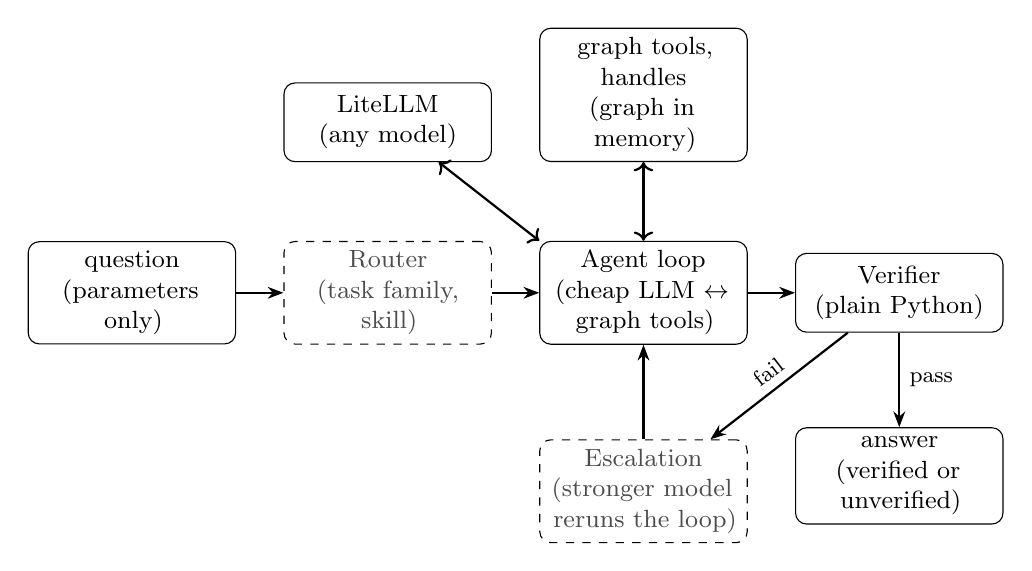
\begin{tikzpicture}[
      node distance=6mm and 6mm,
      box/.style={draw, rounded corners, align=center, minimum height=10mm, text width=24mm, font=\small},
      planned/.style={box, dashed, text=black!70},
      arrow/.style={-{Stealth[length=2mm]}, thick}
    ]
    \node[box] (q) {question\\(parameters only)};
    \node[planned, right=of q] (router) {Router\\(task family,\\skill)};
    \node[box, right=of router] (loop) {Agent loop\\(cheap LLM $\leftrightarrow$\\graph tools)};
    \node[box, right=of loop] (verify) {Verifier\\(plain Python)};
    \node[box, below=12mm of verify] (answer) {answer\\(verified or\\unverified)};
    \node[planned, below=12mm of loop] (esc) {Escalation\\(stronger model\\reruns the loop)};
    \node[box, above=10mm of loop] (tools) {graph tools, handles\\(graph in memory)};
    \node[box, above=10mm of router] (llm) {LiteLLM\\(any model)};

    \draw[arrow] (q) -- (router);
    \draw[arrow] (router) -- (loop);
    \draw[arrow] (loop) -- (verify);
    \draw[arrow] (verify) -- node[right, font=\footnotesize] {pass} (answer);
    \draw[arrow] (verify) -- node[above, sloped, font=\footnotesize] {fail} (esc);
    \draw[arrow] (esc) -- (loop);
    \draw[arrow, <->] (loop) -- (tools);
    \draw[arrow, <->] (llm) -- (loop.north west);
  \end{tikzpicture}
  \caption[Target architecture of the harness]{Target architecture. Solid boxes are built; dashed boxes (router,
  escalation) are planned for M4 and M5. Today the evaluation runner picks the task directly from the dataset, which
  plays the router's role, and a failed verification is sent back to the same model as an error message.}
  \label{fig:architecture}
\end{figure}

A second view, the path of one question through the code as built, is given in Section~\ref{sec:one-question}.

\section{Design principles}

The implementation follows ten principles, fixed at the start of the project. Each is stated below with its
rationale and the way it is realised; deviations are noted.

\paragraph{1. The graph never goes into the prompt.}
The graph lives in Python memory; the model sees only tool results. This removes the dependence of the prompt size on
the graph size and moves the error-prone work (search, counting, copying) into code. For the dataset this means that
questions are rebuilt from a template with only the parameters, because the stored dataset questions contain the full
edge list.

\paragraph{2. Tools never raise.}
Every tool validates its inputs (the node exists, the graph has the right kind, the arguments have the right types)
and returns \texttt{\{"error": ...\}} with a clear, actionable message instead of raising. A crash would end the run;
an error message lets the model correct itself. In an early version, a tool that returned an object instead of a
number crashed the whole run; with this principle in place such bugs become an error message the model can read.

\paragraph{3. Result handles for compaction.}
Large outputs are stored on the harness side, and the model receives a short summary plus an identifier, for example
\texttt{\{"handle": "result\_1", "length": 9932, "first\_5": [...]\}}. Tools and \code{submit_answer} accept handles, so a
9,932-edge spanning forest can be submitted without the model ever writing it out (Section~\ref{sec:handles}). The
principle was later generalised: nothing the model reads may grow with the graph, including error messages and
repeated values.

\paragraph{4. Structured final answers.}
A run ends when the model calls \code{submit_answer}, whose schema depends on the task (a number, true/false, a node
list, an edge list, or a yes/no with evidence). A shape error goes back to the model. The schema matters more than the
instructions: in one experiment, the model was told it could submit a handle, but the schema said ``array'', and it
did the best the schema allowed (Section~\ref{sec:handles}). A second ending tool, \code{cannot_answer}, gives the
model an honest exit instead of a guess.

\paragraph{5. Verification is code, not the model, and checks evidence.}
Each task family has a programmatic verifier. A verifier may check only what the answer itself shows: that a path is
real and connects the right nodes, that a cycle is a cycle, that an edge set is a spanning forest. It must not
recompute the answer and compare it with the submission, because that would be an oracle: accuracy would approach
100\% and any comparison with another harness would be meaningless. Answers that cannot be checked without
re-solving (counts, degrees, edge existence, and every ``no'') are run without a verifier and reported as unverified.
Table~\ref{tab:checkable} summarises the resulting split.

One qualification belongs here. The shortest-path verifier and the waypoint-route verifier check the path against the
graph and then compare its length with the shortest-path distance computed by breadth-first search. The path itself is
evidence, but the optimality check does compute the optimal length. A certificate-based check, in which distance
labels that satisfy every edge prove a length optimal in $O(|E|)$ checks without a search, is noted as a possible
upgrade (\code{docs/gds_agent_findings.md}).
\todo[inline]{Decide whether the BFS length check in verify\_shortest\_path / verify\_path\_via is acceptable under principle 5, or replace it with a distance-label certificate; state the decision here.}

\begin{table}[ht]
  \centering
  \small
  \caption{What can be checked from evidence alone, per task.}
  \label{tab:checkable}
  % source: docs/learning_log.md (2026-10-06), harness/tasks.py, harness/verifiers.py
  \begin{tabularx}{\textwidth}{>{\raggedright\arraybackslash}p{5cm}>{\raggedright\arraybackslash}X}
    \toprule
    Task & Check \\
    \midrule
    \code{shortest_path}, \code{mst}, \code{shortest_path_via} & Full: the answer is the evidence (real edges, right endpoints; no cycle and $n-c$ edges for a spanning forest) \\
    \code{connectivity} ``yes'', \code{cycle_check} ``yes'' & Partial: the model must send the path or cycle, which is checked; a ``no'' is accepted unseen \\
    \code{connected_nodes} & Partial: listed nodes must be real neighbors, each listed once; a missing neighbor cannot be seen \\
    counts, \code{node_degree}, \code{edge_existence}, any ``no'', combine tasks & None: unverified by design \\
    \bottomrule
  \end{tabularx}
\end{table}

\paragraph{6. Show only relevant tools.}
The router picks a task family and the agent sees only that family's tools. Every tool on offer adds to every prompt
and is one more option to choose wrongly. This principle is not yet realised: the router is planned for M4, and today
the model sees all default tools. The cost is visible in the data: adding three tools in M3 grew the tool list the
model reads on every call from about 2,000 to about 2,800 characters.

\paragraph{7. Budgets everywhere.}
Runs have a maximum number of steps (10 by default), a loop detector that stops a run when the model sends the same
reply three times in a row, and, since the context-window problem described in Section~\ref{sec:case-4k}, a stop when
the conversation no longer fits. A maximum cost is part of the principle but is not needed for local models, whose
dollar cost is zero.
\todo[inline]{A per-run dollar budget is not implemented yet; add it before API models are used (M5/M6).}

\paragraph{8. Append-only message history.}
Messages are only appended, which keeps provider prompt caches effective (the prefix of every call is the previous
call). Two deliberate exceptions exist: the model's hidden thinking is removed from its reply before the reply joins
the history (it was otherwise re-sent and re-read on every step), and compaction shortens older tool results near the
context limit, which restarts the cache once.

\paragraph{9. Model-agnostic.}
All model calls go through LiteLLM; no provider is hard-coded. Switching model is changing one string, and the same
loop runs local Ollama models and hosted API models.

\paragraph{10. Log everything.}
Every run writes a JSONL trace: messages, tool calls, results as the model saw them, tokens, latency and, for hosted
models, cost. Every number in Chapter~\ref{ch:results} is reproducible from these files.

\section{Separation of harness and evaluation}

The harness (\code{harness/}) and the evaluation code (\code{eval/}) are separated in one direction: evaluation may
import the harness, never the reverse. The task registry in the harness holds only what the agent may use: the
question template, the answer type and the verifier. Reference answers, dataset parsing and grading live in
\code{eval/tasks.py}, and the grader is written independently of the verifiers. The sandbox that runs model-written
code mounts only the graph file and the harness package, never \code{eval/} or \code{results/}, which hold reference
answers. This is a matter of experimental validity as much as of safety: no ground truth can leak into a run.

A second split concerns the data: graphs 0--49 of each size are the development split, used to build and tune tools,
prompts and routing, and graphs 50--99 are the test split, kept untouched for final results. The split is by graph,
so no test graph is ever seen during development.

\chapter{Implementation}
\label{ch:impl}

This chapter describes the harness as built on 9 October 2026 (milestones M0--M2 complete, M3 steps 1--5 complete).
The description follows \code{docs/architecture.md}, which is kept up to date with the code.

\section{Stack and code organisation}

The harness is written in Python (3.11 or newer) and managed with \code{uv}. Model calls go through LiteLLM
\cite{litellm}; tool arguments and answers are Pydantic models; graph algorithms come from networkx \cite{networkx};
the MCP server uses the official \code{mcp} Python SDK \cite{mcp}; model-written code runs in Docker. Models currently
run locally through Ollama, so there are no API keys in the loop yet; any secrets are read from a git-ignored
\code{.env} file.

\begin{table}[ht]
  \centering
  \small
  \caption{Modules of the harness and the evaluation code.}
  \label{tab:modules}
  % source: docs/architecture.md
  \begin{tabularx}{\textwidth}{>{\raggedright\arraybackslash}p{4.6cm}>{\raggedright\arraybackslash}X}
    \toprule
    File & Job \\
    \midrule
    \code{harness/loop.py} & The agent loop: \code{run_agent}, \code{AgentConfig}, \code{RunResult} \\
    \code{harness/models.py} & One LiteLLM call: tokens, latency, retries, context window \\
    \code{harness/tools/graph_tools.py} & Graph tools, argument models, generated schemas, \code{run_tool} \\
    \code{harness/tools/handles.py} & Result handles and \code{read_result} \\
    \code{harness/tools/mcp_server.py} & The same tools over MCP (stdio) \\
    \code{harness/sandbox/} & \code{run_python}: tool schema, Docker backend, in-container runner, image \\
    \code{harness/compaction.py} & Shortening older messages near the context window \\
    \code{harness/brief.py} & Short versions of values repeated back to the model \\
    \code{harness/answers.py} & Answer types, \code{submit_answer}, \code{cannot_answer}, shape checks \\
    \code{harness/verifiers.py} & Evidence-based checks of final answers \\
    \code{harness/tasks.py} & Task registry: template, answer type, verifier \\
    \code{harness/parsing.py} & Spotting and rescuing tool calls written as text \\
    \code{harness/prompts.py} & All model-facing text and \code{PROMPT_VERSION} \\
    \code{harness/trace.py} & Append-only JSONL trace \\
    \code{eval/tasks.py} & Dataset loading, generated questions, reference answers, grading \\
    \code{eval/runner.py} & Runs the agent over questions, writes \code{results.jsonl} and traces \\
    \code{eval/analysis/report.py} & Accuracy, confidence intervals, tokens, time, code use \\
    \code{eval/analysis/process.py} & Tool precision, recall, F1, parameter match \\
    \code{eval/analysis/trajectory.py} & Classification of how a run reached its answer \\
    \bottomrule
  \end{tabularx}
\end{table}

\section{One question, end to end}
\label{sec:one-question}

The evaluation runner loads a question and its graph, looks up the task in the harness's registry (template, answer
type, verifier) and calls \code{run_agent}. The loop then proceeds as follows.

\begin{enumerate}
  \item The conversation starts with the system prompt and the question. The tools offered are the graph tools, plus
        \code{submit_answer} and \code{cannot_answer}.
  \item Up to the step limit, the model is called with the conversation and the tools.
  \item The model's hidden thinking is removed from its reply before the reply is appended to the history, and logged
        separately.
  \item If the reply contains a tool call written as plain text, the harness either rescues it (parses and runs it,
        lenient mode) or answers with a format error (strict mode). Rescues are counted and logged either way.
  \item If the same reply (text and tool calls, ignoring call identifiers) arrives three times in a row, the run stops
        with status \code{loop_detected}.
  \item Each tool call is handled in turn: arguments that are not a JSON object come back as an error; a graph tool
        is run through \code{run_tool}, which validates the arguments; large values become handles;
        \code{read_result} pages through a handle; \code{submit_answer} resolves any handles, checks the answer's
        shape and then runs the verifier, which either accepts the answer or sends an error back; \code{cannot_answer}
        ends the run.
  \item A reply with no tool call gets a nudge: a format error if it looks like a hand-written tool call, an
        empty-reply message if it has no content at all, and a general nudge otherwise.
  \item Every step is logged to the trace.
\end{enumerate}

The loop returns a \code{RunResult} with the answer, the status (\code{submitted}, \code{cannot_answer},
\code{max_steps}, \code{loop_detected} or \code{context_full}), the evidence, and counters for steps, tokens, model
latency, rescues, rejections and compactions. The runner grades the answer against the reference with
\code{eval/tasks.py}, independently of the verifier, and writes one row to \code{results.jsonl}.

\section{The agent loop}

\subsection{Configuration}

An \code{AgentConfig} holds the settings that stay fixed across the questions of one experiment: the model, the step
limit (default 10), the repeat limit for loop detection (default 3), lenient or strict handling of text tool calls,
which graph tools are offered, which tool functions are available inside code, the handle threshold (default 200
numbers), whether and how \code{run_python} is offered (\code{None}, \code{"tools"} or \code{"networkx"}), whether
the code strategy hint is added to the system prompt, and the compaction threshold (default 75\% of the context
window).

\subsection{Failure handling found by poking the loop}

Several mechanisms in the loop came from early failures of a naive version, observed with qwen3:8b on small graphs
(learning log, 2026-10-04):
\begin{itemize}
  \item Asked for the degree of a node that does not exist, the model read the tool error and then submitted 0,
        because \code{submit_answer} only accepted an integer. The schema shaped the behaviour; the fix was an honest
        exit, \code{cannot_answer(reason)}, logged as its own status rather than as a wrong answer.
  \item Asked for the largest clique with no clique tool, the model first said that the tools were insufficient,
        was nudged twice with a generic ``use the tools or submit'' message, and then guessed. The harness itself had
        caused a hallucination; the nudge now also offers \code{cannot_answer}.
  \item The model wrote \texttt{submit\_answer \{"answer": 0\} </tool\_call>} as plain text nine times until the step
        limit. Feedback now distinguishes a hand-written tool call (\code{FORMAT_ERROR}) from other text
        (\code{NUDGE}), and loop detection ends a run after three identical replies.
\end{itemize}
After these fixes, the clique question ended in \code{cannot_answer} at step~1, and the missing-node question in
\code{cannot_answer} at step~2. The degree question about a missing node gave \code{cannot_answer} in two of four
runs and 0 in the other two: improved, not solved, and a first reminder that one run is not a result.

\subsection{Rescuing text tool calls}

Small models sometimes write a tool call into their text instead of using the function-calling interface. The
harness detects this (tool-call tags, or a tool name followed by a JSON object) and, in lenient mode, parses and runs
the call. Each rescue is logged as a separate event, so that every experiment reports two accuracies: lenient (rescued
answers count) and strict (an answer that needed a rescue counts as wrong). Prose that only mentions a tool name is not
flagged. In the results so far this is the main source of the gap between the two accuracies
(Chapter~\ref{ch:results}).

\subsection{Thinking is not re-sent}

Reasoning models such as qwen3 return their hidden thinking in a separate field of the reply. In an early version the
loop kept that field in the history, so the thinking was sent back and re-read on every later step. Removing it before
the reply joins the history reduced the second-step prompt of one question from 1,826 to 534 tokens. Results before
this fix have inflated prompt tokens on steps after the first; accuracy and output tokens are unaffected.

\section{Tool layer}

\subsection{Tools as validated functions}

Each tool is a plain function \code{tool(graph, **args) -> dict} registered once, together with a Pydantic model for
its arguments and the description the model reads. The JSON schemas shown to the model are generated from the
argument models, and \code{run_tool} validates incoming arguments with the same models, so the schema the model reads
and the validation the harness runs cannot drift apart. When this was introduced, the generated schemas were checked to
be byte-identical to the earlier hand-written ones, so earlier results remained comparable.

Validation produces messages the model can act on, for example ``Bad arguments for shortest\_path: target: Field
required'' or ``node: a node id must be an integer, not true/false''. Two details matter in practice: the string
\code{"3"} is accepted as node 3 (before, it was looked up as a string and reported as missing), and \code{true} is
rejected as a node identifier (Pydantic's lax integer type would have turned it into 1, so node identifiers use a
custom type that refuses booleans). The same strictness applies to answers: in Python a boolean is an integer, so a
number answer rejects booleans and a yes/no answer rejects 0 and 1.

\subsection{The tool set}

There are 13 default tools: \code{get_neighbors}, \code{degree}, \code{has_edge}, \code{graph_info},
\code{shortest_path}, \code{connected_components}, \code{has_cycle}, \code{minimum_spanning_tree}, \code{has_path},
\code{is_bipartite}, \code{topological_sort}, \code{distances_from} and \code{neighborhood}. Five further tools are
opt-in, offered only when requested: \code{articulation_points}, \code{bridges}, \code{k_core}, \code{triangles} and
\code{greedy_coloring}. They came out of the GDS Agent review and are opt-in because every offered tool changes the
prompt, and because \code{triangles} would answer one of the combine tasks in a single call. Appendix~\ref{app:tools}
lists all tools with their arguments and descriptions. New tools are appended, so the text of earlier tools stays the
same.

Where possible, tools return the evidence for their answer, not just the answer: \code{has_cycle} returns one cycle,
\code{has_path} returns a shortest path, \code{is_bipartite} returns the two sides or an odd cycle (so both answers
carry a proof), and \code{topological_sort} returns an order or a directed cycle. The odd cycle comes from the
breadth-first coloring itself: when an edge joins two nodes of the same color, walking both up the BFS tree to their
meeting point gives an odd cycle. When networkx signals ``nothing found'' by raising an exception (no path, no cycle),
the tool turns it into a normal answer such as \code{reachable: false}.

\subsection{Testing against networkx}

Every tool is tested against networkx on all 300 dataset graphs, and the tools without dataset questions (bipartite,
topological sort) also on random graphs, since only 7 small dataset graphs are bipartite and the dataset has no
directed graphs. The tests check the evidence, not only the yes/no. On 9 October 2026 the whole test suite (439 tests)
passes.

\section{Answers and verifiers}

\code{submit_answer} is built per answer type: \code{number}, \code{yes_no}, \code{node_list}, \code{edge_list}, and
\code{yes_no_with_path} and \code{yes_no_with_cycle}, where a ``yes'' carries the path or cycle in an extra field that
is passed to the verifier. The answer itself remains true or false, so grading does not depend on the evidence.

Each verifier has the signature \code{verify(graph, params, answer, **evidence)} and returns either nothing (accept)
or an error message the model can act on. The verifiers are:
\begin{itemize}
  \item \code{verify_shortest_path}: the path starts and ends at the right nodes, every step is an edge, and its
        length equals the shortest-path distance (see the qualification in Chapter~\ref{ch:design}).
  \item \code{verify_mst}: every edge is a real edge, no edge appears twice, the edges contain no cycle (union-find),
        and there are $n-c$ of them for a graph with $n$ nodes and $c$ components. The dataset's graphs are
        unweighted and some are disconnected, so any spanning forest is a correct answer; the old pipeline's checker
        compared against one exact edge set and therefore marked some correct answers wrong.
  \item \code{verify_connectivity} and \code{verify_cycle}: a ``yes'' must come with a real path or a real simple
        cycle of at least three nodes; a ``no'' is accepted unchecked.
  \item \code{verify_neighbors}: every listed node is a real neighbor and is listed once; a missing neighbor cannot be
        detected.
  \item \code{verify_path_via}: a real route from source to target through the waypoint, whose length equals the sum
        of the two shortest-path distances.
\end{itemize}

\section{Result handles and bounded messages}
\label{sec:handles}

\subsection{Handles}

A value with more than 200 numbers is stored in a per-run \code{HandleStore}, and the model sees a summary with an
identifier, the length and the first five items. A list of large items, such as the components of a graph, gets one
handle per item. Once a handle exists, \code{read_result(handle, offset, limit)} is offered, and \code{submit_answer}
accepts a handle string in place of the value. Before that, the tool list is unchanged, so the current dataset, whose
largest tool output has 98 numbers, never sees handles and earlier results are unaffected.

The first real test illustrates principle 4. On a random graph with 10,000 nodes, 25,000 edges and 68 components,
qwen3:8b was asked for a minimum spanning tree (the answer has 9,932 edges). The tool result came back as a
336-character summary instead of about 110,000 characters, as intended. The model then submitted the handle twice,
was rejected both times, and gave up, explaining that the system required the actual list of edges. The note said
``pass the handle to submit\_answer'', but the schema of \code{submit_answer} said the answer must be an array of
edges, so a string was impossible. After the fix (once a handle exists, the schema becomes ``edge list or a handle
string'', and a handle wrapped in a list is resolved too), the same question took two steps, 35 seconds and 1,974
prompt plus 601 completion tokens, and the verifier checked all 9,932 edges.
% source: docs/learning_log.md (2026-10-07, M3 step 3), results/harness_runs/handles_big_graph_test

\subsection{Nothing the model reads grows with the graph}

Handles only cover tool results. A review found other messages that scaled with the graph: the missing-node error
listed every node identifier, about 59,000 characters on a 10,000-node graph for a single typo. It now reads ``Node
123456 does not exist. G has 10000 nodes, with ids 0 to 9999.'' An audit of every formatted message then produced
Table~\ref{tab:bounded}. The fix is a helper, \code{brief()}, used wherever a value is repeated to the model, and a
test file that checks every such message on a 10,000-node graph.

\begin{table}[ht]
  \centering
  \small
  \caption{Size of messages that repeat a value back to the model, on a 10,000-node graph, before and after the audit.}
  \label{tab:bounded}
  % source: docs/learning_log.md (2026-10-08, missing-node errors and follow-up audit)
  \begin{tabularx}{\textwidth}{>{\raggedright\arraybackslash}X r >{\raggedright\arraybackslash}p{5cm}}
    \toprule
    Message & Before (characters) & After \\
    \midrule
    Wrong-type answer repeated in full & 174,455 & about 280 (first items and size) \\
    A page of large items from \code{read_result} & 69,676 & about 3,500 (each big item its own handle) \\
    The whole cycle repeated by the cycle verifier & 28,923 & names the repeated node \\
    Missing node: every node listed & about 59,000 & 66 \\
    Unknown handle: every stored handle listed & 438 (grows) & first 10 and a count \\
    \bottomrule
  \end{tabularx}
\end{table}

\section{The MCP server}

The MCP server (\code{harness/tools/mcp_server.py}) gives other harnesses exactly our tools. It uses the official
\code{mcp} SDK's low-level server: the tool list is built from the same generated schemas (same names, descriptions
and schemas), calls go through \code{run_tool} (same validation and errors, flagged as errors in MCP), and large results
become handles. The SDK's own argument validation is switched off so that error messages match our loop. The server
speaks stdio, and the client launches one server process per question with the graph file as an argument, so handles
never leak between questions. Differences from our loop: \code{read_result} is listed from the start, and
\code{submit_answer} is not served yet; how a general-purpose harness should submit structured answers is decided in
M6. Our own loop does not use MCP; it calls \code{run_tool} directly.

FastMCP was considered and not used: its main convenience, schemas generated from function signatures, is the opposite
of what is needed, which is our schemas byte for byte. The server is an adapter of about a hundred lines. Nine tests
check that the tool list equals ours, that every tool's result through MCP equals \code{run_tool} on dataset graphs,
that errors match, that handles work, and that the server runs as a real subprocess over stdio.
\todo[inline]{Open decision recorded in CLAUDE.md: keep the mcp package as a project dependency (it is in pyproject.toml now).}

\section{The run\_python sandbox}

\subsection{Design}

\code{run_python} lets the model write code. It is off by default and offered in one of two modes. In
\code{"tools"} mode, the code sees our graph tools as plain Python functions and cannot import networkx, so it
composes our tools instead of bypassing them and their evidence. In \code{"networkx"} mode, the code also gets the
graph \code{G} and \code{nx}: the escape hatch, kept for comparison.

The code runs in a Docker container, one per question, started on the first call (about 0.3 seconds) and reused for
later calls (about 0.3 milliseconds per call), so variables persist between calls. The container has no network, a
read-only file system except a small \code{/tmp}, 512~MB of memory, one CPU, at most 64 processes, no capabilities, a
non-root user, and 10 seconds per call, after which it is killed and restarted and the reply says that variables were
lost. Only the graph file and the \code{harness/} package are mounted, read-only. The model gets back the value of
\code{result} (large values become handles), the printed output (shortened), and errors in the form ``line 2:
IndexError: list index out of range'', pointing at the model's line rather than at harness internals. The backend is
swappable; a WebAssembly backend that needs no Docker is the plan for a public release. On the MacBook, Docker is
provided by OrbStack; on the GPU machine by Docker Engine.
\todo[inline]{Open decision recorded in CLAUDE.md: Docker vs OrbStack/Colima for the sandbox on macOS.}

\subsection{Plain values in code}

The first version exposed the tools inside code exactly as the model sees them in the loop, returning JSON
dictionaries. That failed: \code{for n in get_neighbors(4)} iterated over the dictionary's keys, and an error
dictionary flowed on as if it were a result. Inside code the tools now return plain values, as networkx does
(\code{get_neighbors(4)} returns \code{[2, 5]}; \code{shortest_path(a, b)} returns a path or \code{None}), and tool
errors raise \code{ValueError}. \code{graph_info()} and \code{is_bipartite()} keep their dictionaries, and the tool
description shows what \code{graph_info()} returns. If the model redefines a tool function (one run defined
\code{get_neighbors} in terms of itself and broke every later call), the original is restored after the call, with a
note. The lesson recorded at the time: an interface the model already knows beats a better one it has to learn, so
ours was made to look familiar.

\section{Context window and compaction}

\subsection{The context window}

Ollama serves every model with a 4,096-token context unless asked otherwise, regardless of what the model supports.
Past that limit the prompt is cut and the reply stops short, with no error. This silently damaged one family of
experiments (Section~\ref{sec:case-4k}). The model layer now asks Ollama for 16,384 tokens, logs the context window in
every run's first trace event, and flags any prompt above 90\% of it. Hosted models keep the provider's context.

\subsection{Compaction}

When a prompt passes 75\% of the window, the loop shortens the conversation before the next call, by fixed rules and
without an LLM summary (free and reproducible). Older tool results longer than 300 characters become a short version
with a note (``shortened; call the tool again for the full result''), older \code{run_python} code longer than 200
characters is cut to its start, and the system prompt, the question and the last two rounds stay word for word. No
message is deleted, because the chat format requires every tool call to keep its reply, and handles keep their full
values in the store. Each compaction is logged and counted. If nothing is left to shorten and the prompt is above
90\%, the run ends with status \code{context_full} instead of continuing with a cut prompt. The cost is that the
provider's prompt cache restarts once after a compaction, because the prefix has changed. In the runs reported in
Chapter~\ref{ch:results}, no conversation was compacted.

\section{Prompt versioning}

Every piece of text the harness says to the model lives in \code{harness/prompts.py}, together with
\code{PROMPT_VERSION}, which is logged in every run. The version is bumped, with a changelog line, whenever any
model-facing text changes, including tool descriptions. Table~\ref{tab:prompt-versions} summarises the changelog.
Appendix~\ref{app:prompts} reproduces the current texts.

\begin{table}[ht]
  \centering
  \small
  \caption{Prompt versions (changelog in \code{harness/prompts.py}).}
  \label{tab:prompt-versions}
  % source: harness/prompts.py (PROMPT_VERSION changelog)
  \begin{tabularx}{\textwidth}{l>{\raggedright\arraybackslash}X}
    \toprule
    Version & What changed \\
    \midrule
    v1 & Everything up to and including the M2 pilots \\
    v2 & v1 plus \code{distances_from} and \code{neighborhood}; used by the M2 closing runs and the Claude Code comparison on large graphs \\
    v3 & Merge of the two machines' work: Pydantic schemas, three new tools, result handles, bounded messages, waypoint question \\
    v4 & \code{run_python} description: plain values, errors raise, do not redefine tools \\
    v5 & \code{CODE_HINT} (strategy hint, only with \code{run_python} and the hint on); combine-task wording \\
    v6 & \code{EMPTY_REPLY} nudge; \code{graph_info()} shown in the \code{run_python} description; redefined tools restored \\
    v7 & Compaction texts; runs that never approach the limit see the same text as v6 \\
    \bottomrule
  \end{tabularx}
\end{table}

\section{Logging and analysis}

\subsection{Traces and results}

Every run writes the events \code{run_start} (configuration, prompt version, context window), \code{model_call}
(content, tool calls, thinking, tokens, latency), \code{tool_call} (arguments and the result as the model saw it),
\code{rescued_tool_call}, \code{verifier_rejected}, \code{nudge}, \code{compacted} and \code{run_end} to
\code{traces.jsonl}, and one row per answer to \code{results.jsonl}. An early version of the runner re-read the whole
trace file after every question to find that question's token counts, which made the work grow quadratically with the
number of questions; the loop now returns these counts directly. The log is for later analysis, not for passing data
between parts of the program.

\subsection{The report}

\code{eval/analysis/report.py} puts experiments side by side, overall and per task: lenient and strict accuracy, a 95\%
bootstrap confidence interval over questions (all runs of a question are resampled together), the share of answers a
verifier actually looked at, the number of answers sent back by a verifier, runs without an answer, compactions, and
tokens and time per question. With \code{--code} it reports how \code{run_python} was used, and with \code{--process}
the process metrics below. All tables in Chapter~\ref{ch:results} are produced by this script.

\subsection{Process metrics}
\label{sec:process-metrics}

\code{eval/analysis/process.py} measures whether the model called the right tools with the right arguments, using the
definitions of the GDS Agent benchmark \cite{gdsagentbench}. For each task, \code{EXPECTED_CALLS} lists the calls an
ideal run makes; each expected call is a slot that one of several equivalent tools can fill (for example, a node's
degree from \code{degree} or from \code{get_neighbors}). With $E$ expected calls, $M$ of them made, and $T$ scored tool
calls in the run:
\begin{align*}
  \text{recall} &= M / E, &
  \text{precision} &= M / T, &
  F_1 &= \frac{2PR}{P + R}.
\end{align*}
Repeating a call or exploring lowers precision. Parameter match is the share of right arguments in the expected calls
that were made directly, and exact match means every expected call was made and nothing else. Three deliberate
differences from the original definitions follow from our setup: \code{run_python} counts as one tool call and fills
an expected slot when its code calls that tool function (its arguments cannot be read, so it adds no parameter score);
argument pairs $(u, v)$ and (source, target) also match when swapped, since all graphs are undirected; and the
parameter score takes the best matching call, since the waypoint task makes the same tool call twice. The ending tools
and \code{read_result} are not scored.

\subsection{Trajectory analysis}

For multi-step tasks, \code{eval/analysis/trajectory.py} classifies each run by its graph tool calls and its answer:
ideal, extra calls, alternative path (different calls, correct answer), right calls but wrong answer, or wrong path,
with flags for detours such as taking the shortcut, using \code{has_path} for a leg, or exploring manually with
\code{get_neighbors}. The ``alternative path'' class exists because the first version labelled a correct and well
reasoned run as incomplete; process evaluation has to judge whether each step is justified, not whether it matches one
expected sequence.

\chapter{Experimental Setup}
\label{ch:setup}

This chapter describes the data, the models and hardware, the configurations compared, and the metrics. It also
states the limits of the current setup, which apply to every result in Chapter~\ref{ch:results}.

\section{Dataset}

\subsection{Graphs and problems from the prior work}

The experiments so far reuse the dataset of the prior work \cite{skianis2024pseudocode}, generated by
\code{scripts/generate_dataset.py} and stored in \code{data/graphs/} and \code{data/graphs_questions/}. It contains
Erd\H{o}s--R\'enyi graphs in three sizes, 100 graphs per size (300 in total): small graphs with 5--10 nodes, medium
graphs with 11--20 nodes and large graphs with 21--50 nodes. For each graph the generator draws the edge probability
uniformly from $[0, 1]$, removes isolated nodes and self-loops, and redraws until the graph has the intended number of
nodes. All graphs are undirected and unweighted, and five small graphs are disconnected, so a ``minimum spanning
tree'' there is any spanning forest.

The ten problems are node count, edge count, node degree, neighbors of a node (\code{connected_nodes}), edge
existence, connectivity between two nodes, number of connected components, cycle check, shortest path, and minimum
spanning tree. The harness keeps only the parameters of each stored question (node identifiers) and rebuilds the
question from its own template (Table~\ref{tab:templates} in Appendix~\ref{app:tools}), because the stored questions
contain the full edge list. Topological sort and bipartiteness have tools but no questions yet; they come with the
scaled generator of M6.

\subsection{An audit of the dataset}
\label{sec:audit}

Counting on the development graphs showed that several tasks have, in practice, one possible answer
(Table~\ref{tab:audit}). The large graphs are very dense, between 63 and 1,005 edges on 21--50 nodes, so paths are
short (the average shortest-path length in the large questions is 1.5, at most 3) and almost every pair of nodes is
connected by an edge. A model that always answers ``yes'' or ``1'' would score about 100\% on edge existence, cycle
check and component count on the large graphs. These tasks still test whether the loop and tools work, but they
cannot separate a good model from a lucky one. Only connectivity on small graphs is balanced, and there are no
connectivity questions for large graphs at all.

The large graphs are a real test in three places: \code{connected_nodes} (on average 21 and up to 45 neighbors to
list), \code{node_degree} (counting up to 45), and \code{mst} (on average 36 and up to 49 edges to list). Those are the
tasks where copying mistakes, and the effect of verifiers, can show.

\begin{table}[ht]
  \centering
  \small
  \caption{Answer balance on the development graphs (0--49).}
  \label{tab:audit}
  % source: docs/learning_log.md (2026-10-06, dataset audit)
  \begin{tabular}{lrr}
    \toprule
    & small (5--10 nodes) & large (21--50 nodes) \\
    \midrule
    \code{edge_existence} answer is ``yes'' & 97 / 100 & 100 / 100 \\
    graph has a cycle & 47 / 50 & 50 / 50 \\
    graph is connected (one component) & 47 / 50 & 50 / 50 \\
    connectivity questions (yes / no) & 28 (14 / 14) & 0 \\
    shortest-path length & -- & average 1.5, maximum 3 \\
    \bottomrule
  \end{tabular}
\end{table}

Two consequences follow for the thesis: per-task accuracy should be reported next to a majority-answer baseline, so
that 100\% on a one-answer task is read correctly, and the M6 generator should balance yes/no answers and control
density, so that paths are long and not every pair is an edge.
\todo[inline]{Add the majority-answer baseline column to the report (planned, not implemented yet).}

\subsection{Generated tasks}

Four tasks have no questions in the dataset; their questions are generated from the development graphs with a fixed
seed per task, size and graph, so that every run sees the same questions.

\paragraph{Waypoint route (\texttt{shortest\_path\_via}).} ``What is the shortest route from node A to node B if it must
pass through node C?'' No single tool answers it: the ideal run calls \code{shortest_path(A, C)} and
\code{shortest_path(C, B)} and joins the two paths. The generator only keeps waypoints that force a detour, so the
shortcut \code{shortest_path(A, B)} is always wrong, and sometimes the best route revisits a node. It is fully
verified.

\paragraph{The combine family.} Three tasks that need one lookup to find candidates and then many lookups and a
comparison:
\begin{itemize}
  \item \code{hop_max_degree}: among the nodes within $k$ hops of a node, which has the highest degree (ties to the
        smallest identifier); $k = 1$ on the dense large graphs, where two hops already reach almost every node;
  \item \code{common_neighbors_max}: which other node shares the most neighbors with a given node;
  \item \code{triangle_count}: how many triangles include a given node.
\end{itemize}
The questions pick a node with at least three neighbors, so there is something to loop over. With tools alone these
tasks need dozens of calls; one loop in code over the tool functions does it in one step. Their answers are numbers,
so they are unverified by design.

\paragraph{Multi-step probes.} Two hand-written questions (``which node is farthest from node 0?'' and ``how many other
nodes are within 2 hops of node 5?'') were used once to test the \code{distances_from} and \code{neighborhood} tools.

\section{Development and test split}

Graphs 0--49 of each size are the development split and graphs 50--99 the test split. Tools, prompts and routing are
designed on the development split only. Every result in this draft is on the development split; the test split has
not been used.

\section{Models and hardware}

\subsection{Local models}

All harness runs so far use local models served by Ollama and called through LiteLLM: \code{qwen3:8b} (the default
cheap model so far) and \code{qwen3.5:9b} (used for the combine experiments). The model's default temperature is used;
no temperature has been set.
\todo[inline]{Decide and fix the sampling temperature before the final experiments, and report it.}

Real runs are made on a machine with an NVIDIA RTX 5070 with 12~GB of memory, where a simple question takes about 4
seconds. A MacBook Air with an M4 chip and 24~GB of memory also runs qwen3:8b, but about 4.5 times slower (about 30
seconds per answer in the pilot), and is used only for quick tests. Which machine a result comes from is stated with
it. Since 8 October 2026, every Ollama call requests a 16,384-token context; earlier runs used Ollama's default of
4,096 tokens (Section~\ref{sec:case-4k}).

The choice of the cheap model is not final. A pilot of four candidates that fit the 12~GB GPU is planned
(Table~\ref{tab:candidates}), each on 54 questions (all nine large-graph tasks, six questions each, one run), to
decide on strict accuracy, rescued tool calls, verifier rejections, and tokens and time per question.

\begin{table}[ht]
  \centering
  \small
  \caption{Candidate models for the planned pilot. Sizes are from model pages and blogs and are unverified.}
  \label{tab:candidates}
  % source: CLAUDE.md ("Model candidates"), docs/learning_log.md (2026-10-08, model choice)
  \begin{tabularx}{\textwidth}{l>{\raggedright\arraybackslash}X>{\raggedright\arraybackslash}p{3.5cm}}
    \toprule
    Model & Why & Fits 12 GB? \\
    \midrule
    \code{qwen3.5:9b} & Likely new default: successor to qwen3:8b, same memory (6.6--7.6 GB) & yes \\
    \code{gemma4:12b} & A second model family, native function calling, 7.7--8 GB & yes \\
    \code{gpt-oss:20b} & Strong function calling; 14 GB download, sources disagree on fit & to test \\
    \code{qwen3:8b} & Current baseline, rerun with today's tool set & yes \\
    \code{qwen3.6:35b-a3b} & Strongest local option (mixture of experts, 3B active) for M5 escalation & offload only \\
    \bottomrule
  \end{tabularx}
\end{table}

Hosted models are planned as stronger baselines in our harness: a frontier closed model and a strong open model
through an API.
\todo[inline]{Fix the hosted models (CLAUDE.md lists Sonnet 5.5 and Kimi K2.6 via OpenRouter) and the API access; there is no API access yet.}

\subsection{The general-purpose harness}

The comparisons with a general-purpose harness use Claude Code in headless mode (\code{claude -p}) with a Sonnet
model on a subscription; the reported dollar cost is the API-equivalent cost that Claude Code reports. Two setups were
used. In the first, Claude Code may only run the project's Python (with networkx) and read the graph file, and answers
with JSON on its last line. In the second, all of Claude Code's built-in tools are switched off and it sees only our
tools through the MCP server; it is run outside the repository so that no project instructions are loaded. In one run
the alias \code{sonnet} resolved to a different model version than intended, so model identifiers must be pinned in
the M6 baselines.

\section{Configurations}

\paragraph{Lenient and strict.} Every run is lenient (text tool calls are rescued), and the strict accuracy is computed
from the same run by counting every answer that needed a rescue as wrong.

\paragraph{Verifiers on and off.} With \code{--no-verify} the model is still asked for the same answers with the same
evidence fields; only the checking is switched off.

\paragraph{Tool ablations.} \code{--without-tool} removes a tool from the default set (for example \code{has_edge} or
\code{degree}) and \code{--with-tool} adds an opt-in tool. Because the default tool set grew during the project,
results from different dates are not directly comparable; each experiment states its tool set or prompt version.

\paragraph{Code versus tools.} Five setups compare tool calls with code on the combine tasks (Table~\ref{tab:setups}).
Setup B offers \code{run_python} next to the tools; setup H adds the strategy hint \code{CODE_HINT} to the system
prompt (``use a direct tool for a single lookup; when the answer needs many lookups, write one \code{run_python} call
that loops over the tool functions''); setup C offers code only, with our tools as functions; setup NX offers code
only, with networkx.

\begin{table}[ht]
  \centering
  \small
  \caption{Setups of the code-versus-tools experiments.}
  \label{tab:setups}
  % source: results/harness_runs/combine16k_qwen35_*/traces.jsonl (run_start), docs/architecture.md
  \begin{tabularx}{\textwidth}{l>{\raggedright\arraybackslash}X l l}
    \toprule
    Setup & Offered & \code{python} & hint \\
    \midrule
    A & Graph tools only & off & no \\
    B & Graph tools and \code{run_python} (tool functions inside code) & \code{tools} & no \\
    H & As B, plus \code{CODE_HINT} in the system prompt & \code{tools} & yes \\
    C & \code{run_python} only, tool functions inside code, no networkx & \code{tools} & no \\
    NX & \code{run_python} only, with \code{G} and \code{nx} (networkx) & \code{networkx} & no \\
    \bottomrule
  \end{tabularx}
\end{table}

\section{Metrics}

\begin{itemize}
  \item \emph{Accuracy} (lenient): the share of all answers, over every run, graded correct by \code{eval/tasks.py}.
        The grader accepts any shortest path, neighbors in any order, any spanning forest, and never counts
        \code{true} as 1.
  \item \emph{95\% confidence interval}: bootstrap over questions, with all runs of a question resampled together.
  \item \emph{Strict accuracy}: accuracy without answers rescued from text tool calls.
  \item \emph{Checked}: the share of answers a verifier actually looked at; \emph{rejected}: answers a verifier sent
        back; \emph{no answer}: runs that ended without one (\code{cannot_answer}, loop detected, step limit, context
        full, error).
  \item \emph{Cost}: prompt plus completion tokens per answer, and wall-clock time per answer. The dollar cost of local
        runs is zero; for Claude Code the reported API-equivalent cost is used.
  \item \emph{Process metrics}: tool precision, recall, F1, parameter match and exact match
        (Section~\ref{sec:process-metrics}), as in the GDS Agent benchmark.
  \item \emph{Code use}: the share of questions with at least one \code{run_python} call, with both code and graph
        tools, code calls and graph-tool calls per question, the share of code calls that ended in an error, and
        empty replies.
\end{itemize}

The primary comparison of the thesis, the accuracy-versus-cost Pareto front, combines accuracy with tokens, time and
dollars. No Pareto analysis has been done yet; it needs the hosted-model baselines and repeated runs (M7).

\section{Limitations of the current setup}

The results in Chapter~\ref{ch:results} should be read with these limitations in mind:
\begin{itemize}
  \item Most experiments are a single run, many on 3--15 questions; the plan requires at least three runs per
        configuration. With 15 questions, one question is 6.7 percentage points.
  \item Confidence intervals are reported where the report computes them, but with one run and few questions they
        are wide, and for tasks at 100\% the bootstrap interval collapses to a point.
  \item All results are on the development split, which was also used to design the tools and prompts.
  \item The existing dataset is saturated on large graphs (Section~\ref{sec:audit}); it cannot yet separate setups on
        most tasks.
  \item The tool set and prompt version changed between experiments, so experiments from different dates are not
        directly comparable.
  \item The comparisons with Claude Code use a different model and, in one case, different tools; they are
        previews, not the fair comparison planned for M6.
  \item The temperature was left at the model default.
\end{itemize}

\chapter{Results So Far}
\label{ch:results}

This chapter reports every experiment run up to 9 October 2026, roughly in the order they were made. All of them are on
the development split. Most are a single run on a handful of questions, made while the harness was being built, and
several were made to decide a design question rather than to measure the final system. They show where the harness
stands and what each component did when it was introduced; they do not yet answer the research question. Unless
stated otherwise, tables are produced by \code{eval/analysis/report.py} from the folder named in the caption, and the
model is \code{qwen3:8b}.

\section{First experiment: node degree on small graphs}

The first experiment asked 100 node-degree questions on the small development graphs (two per graph), with only two
tools available, \code{get_neighbors} and an edge counter, and no edge list in the prompt. It was planned as three
runs; the third was stopped after 12 questions. Over the 212 answers, accuracy was 99.5\% (95\% CI 98.6--100\%), at
about 1,356 tokens and 4.3 seconds per answer. The only failure was not a reasoning failure: the model called
\code{get_neighbors}, received the six neighbors, and then wrote its (correct) answer of 6 as a text tool call three
times, until loop detection stopped the run. This was the first sign that the final answer's format, not the
reasoning, would be the cheap model's weak point.
% source: results/harness_runs/degree_small_dev_v1, docs/learning_log.md (2026-10-04)

\section{Well-fitting tools}

Three times during the project a tool was added that answers a task directly, and each time the effect was the same.

\subsection{A direct edge test}

Table~\ref{tab:has-edge} compares five edge-existence questions on small graphs with and without \code{has_edge}.
Without it, the model spent 1,500--2,700 thinking tokens working out that \code{get_neighbors} answers the question
before making its first call; with it, 275--287 tokens every time.

\begin{table}[ht]
  \centering
  \small
  \caption[Ablation: the has\_edge tool]{Ablation of \code{has_edge}: 5 edge-existence questions, small development
  graphs, 1 run. Prompt tokens in these runs are inflated by the thinking-in-history bug (fixed later); accuracy and
  output tokens are unaffected.}
  \label{tab:has-edge}
  % source: results/harness_runs/has_edge_ablation_without, results/harness_runs/has_edge_ablation_with, docs/learning_log.md (2026-10-05)
  \begin{tabular}{lrr}
    \toprule
    & without \code{has_edge} & with \code{has_edge} \\
    \midrule
    correct & 5/5 & 5/5 \\
    output tokens (all 5 questions, mostly thinking) & 2,256 & 282 \\
    prompt tokens (all 5 questions) & 4,200 & 1,231 \\
    tokens per question (report) & 6,456 & 1,514 \\
    time per question & 23.7 s & 3.1 s \\
    \bottomrule
  \end{tabular}
\end{table}

\subsection{A degree tool}

In the large-graph pilot, node-degree questions were by far the slowest (133 seconds per answer on the MacBook,
up to 223 seconds). The time went into the first step, before any tool call: the model debated whether $G$ might be
directed and the degree therefore in-degree plus out-degree, then called \code{graph_info} to check. Its first thought
was that there is no function called degree, so \code{get_neighbors} was the way to go. Adding \code{degree}
(Table~\ref{tab:degree}) removed both the debate and the counting.

\begin{table}[ht]
  \centering
  \small
  \caption[Ablation: the degree tool]{Ablation of \code{degree}: the same 6 node-degree questions on large development
  graphs, 1 run, MacBook Air M4.}
  \label{tab:degree}
  % source: results/harness_runs/m2_pilot_large_verify, results/harness_runs/degree_tool_large_pilot, docs/learning_log.md (2026-10-07)
  \begin{tabular}{lrr}
    \toprule
    & without \code{degree} & with \code{degree} \\
    \midrule
    correct & 6/6 & 6/6 \\
    time per question & 133 s (max 223 s) & 17 s (max 23 s) \\
    output tokens (mostly thinking) & 1,988 & 264 \\
    total tokens & 3,758 & 1,582 \\
    rescued text tool calls & 4/6 & 1/6 \\
    \bottomrule
  \end{tabular}
\end{table}

\subsection{Building blocks for multi-step questions}

Two questions that no single tool answered, the farthest node from a given node and the number of nodes within two
hops, were asked on one small graph (7 nodes) and one large graph (29 nodes), first with the basic tools and then with
\code{distances_from} and \code{neighborhood} added (Table~\ref{tab:multistep}). These runs were not traced; the
numbers come from the console output recorded in the learning log.

\begin{table}[ht]
  \centering
  \small
  \caption{Multi-step probes with and without the building-block tools (1 run each, not traced).}
  \label{tab:multistep}
  % source: docs/learning_log.md (2026-10-07, multi-step questions)
  \begin{tabularx}{\textwidth}{l>{\raggedright\arraybackslash}X>{\raggedright\arraybackslash}p{4cm}}
    \toprule
    Question & Basic tools & With \code{distances_from}, \code{neighborhood} \\
    \midrule
    small, farthest & correct; 7 steps, 70 s (components, then 4 shortest paths) & correct; 2 steps, 20 s \\
    small, within 2 hops & gave up with no tool call, 87 s & correct; 2 steps, 10 s \\
    large, farthest & gave up after one shortest-path call & correct; 2 steps, 16 s \\
    large, within 2 hops & answered 26 (truth 28) after 4 of the needed neighbor calls, 151 s & correct; 2 steps, 9 s \\
    \bottomrule
  \end{tabularx}
\end{table}

With low-level tools the model would have needed about 28 calls and the merging of lists in its head, so it gave up
or did part of the work and guessed. The new tools were not written for these exact questions: they also answer ``how
many nodes at distance 3'', ``is anything unreachable'', eccentricity, and any $k$-hop question. Two side observations:
\code{cannot_answer} stopped the guessing but became an easy way out on questions the model could have answered, and
the wrong answer of 26 looked as confident as a correct one, because these question types have no verifier.

\section{M2 closing run: verifiers on and off}

\subsection{Pilot}

A pilot on the MacBook (large development graphs, all nine tasks with large questions, six questions each, one run,
verifiers on) answered all 54 questions correctly in lenient mode and 43 of 54 (79.6\%) in strict mode. In every
question the model picked the right tool on its first call. Eleven answers (20\%) were rescued text tool calls, and in
five of six cycle-check questions the verifier sent the answer back once, because the model answered ``yes'' without
the cycle. Its thinking showed why: the cycle was in the tool result, but ``the user only asked if there's a cycle, so
confirming true is sufficient''. The description of \code{submit_answer} makes the evidence sound optional.
% source: results/harness_runs/m2_pilot_large_verify, docs/learning_log.md (2026-10-07, pilot)

\subsection{Closing run}

The closing run of M2 was made on the RTX 5070 with the large development graphs: nine tasks, 15 questions each, two
runs, prompt version v2, once with verifiers (\code{m2_large_verify}) and once without (\code{m2_large_noverify}).
Without verifiers the model is still asked for the same evidence; only the checking is off. The two fixes suggested by
the pilot (saying that evidence is required, and stating in the prompt that $G$ is undirected) were not applied first.
Table~\ref{tab:m2} gives the overall numbers and Table~\ref{tab:m2-tasks} the strict accuracy per task.

\begin{table}[ht]
  \centering
  \small
  \caption{M2 closing run: large development graphs, 9 tasks $\times$ 15 questions $\times$ 2 runs, qwen3:8b, RTX 5070.}
  \label{tab:m2}
  % source: results/harness_runs/m2_large_verify, results/harness_runs/m2_large_noverify
  % (uv run python -m eval.analysis.report m2_large_verify m2_large_noverify --by-task)
  \begin{tabular}{lrr}
    \toprule
    & verifiers on & verifiers off \\
    \midrule
    answers & 270 & 270 \\
    accuracy (lenient) & 100.0\% & 100.0\% \\
    strict accuracy & 88.1\% & 90.4\% \\
    answers a verifier looked at & 44\% & 0\% \\
    answers sent back by a verifier & 18 & -- \\
    runs without an answer & 0 & 0 \\
    tokens per question & 2,237 & 2,145 \\
    time per question & 4.6 s & 4.3 s \\
    \bottomrule
  \end{tabular}
\end{table}

\begin{table}[ht]
  \centering
  \small
  \caption[M2 closing run per task]{M2 closing run per task. Lenient accuracy is 100\% for every task in both
  conditions; the table shows strict accuracy, tokens and time per question.}
  \label{tab:m2-tasks}
  % source: results/harness_runs/m2_large_verify, results/harness_runs/m2_large_noverify (report --by-task)
  \begin{tabular}{lrrrrrr}
    \toprule
    & \multicolumn{3}{c}{verifiers on} & \multicolumn{3}{c}{verifiers off} \\
    \cmidrule(lr){2-4}\cmidrule(lr){5-7}
    Task & strict & tokens & time & strict & tokens & time \\
    \midrule
    \code{connected_components_count} & 96.7\% & 2,081 & 3.4 s & 96.7\% & 2,068 & 3.2 s \\
    \code{connected_nodes} & 46.7\% & 2,368 & 5.2 s & 60.0\% & 2,135 & 4.2 s \\
    \code{cycle_check} & 93.3\% & 2,797 & 5.0 s & 96.7\% & 2,121 & 3.9 s \\
    \code{edge_count} & 100.0\% & 1,930 & 3.2 s & 100.0\% & 1,952 & 3.3 s \\
    \code{edge_existence} & 100.0\% & 1,934 & 3.5 s & 100.0\% & 1,965 & 3.1 s \\
    \code{mst} & 83.3\% & 3,128 & 11.0 s & 83.3\% & 3,163 & 11.0 s \\
    \code{node_count} & 93.3\% & 1,980 & 3.7 s & 96.7\% & 1,982 & 3.7 s \\
    \code{node_degree} & 100.0\% & 1,875 & 2.7 s & 90.0\% & 1,875 & 2.7 s \\
    \code{shortest_path} & 80.0\% & 2,042 & 3.6 s & 90.0\% & 2,046 & 3.6 s \\
    \bottomrule
  \end{tabular}
\end{table}

Four observations follow.
\begin{enumerate}
  \item The verifiers never caught a wrong answer, because there were none: the tools compute the answer and the
        model copies it correctly. On these tasks the verifiers cost a little (4\% more tokens) and bought nothing.
  \item All 18 rejections were the same: a ``yes'' to cycle check without the cycle (18 of 30 cycle-check runs), each
        fixed on the second try. This made cycle check 32\% more expensive in tokens (2,797 against 2,121) and about
        1.1 seconds slower. It is the pilot's finding again, and the open fix A (evidence required) targets it.
  \item Rescued text tool calls are the real error source: 10--12\% of answers. They concentrate in
        \code{connected_nodes}, where 16 of 30 and 12 of 30 answers were rescued, about half, and then in shortest
        path and MST: the tasks whose answers are long lists.
  \item The large dataset graphs no longer separate anything: every task is at 100\% lenient accuracy with the
        current tools. The confidence intervals in the report are degenerate (100--100\%) for the same reason.
\end{enumerate}
The differences in strict accuracy between the two conditions (for example 46.7\% against 60.0\% on
\code{connected_nodes}) come from 30 answers per cell and one pair of runs each, and should not be read as an effect
of the verifiers: the verifier only runs after an answer has been submitted, rescued or not.

\subsection{Process metrics}

Scored with the process metrics of Section~\ref{sec:process-metrics}, both M2 runs are process-perfect: tool precision,
recall and F1 of 1.00, parameter match 1.00 and exact match 100\% over all 270 answers each. On these nine tasks the
cheap model always called the one expected tool with the right arguments, and nothing else.
% source: results/harness_runs/m2_large_verify, results/harness_runs/m2_large_noverify (report --process)

\section{Large graphs: result handles}

The handle mechanism was tested on one generated graph with 10,000 nodes, 25,000 edges and 68 components
(Section~\ref{sec:handles}). After the schema fix, qwen3:8b answered the minimum-spanning-tree question in two steps,
35 seconds and 1,974 prompt plus 601 completion tokens, by submitting the handle of the tool result, and the verifier
checked all 9,932 edges. Without handles, the tool result alone would have been about 110,000 characters. This is a
single run on a single graph; size scaling is planned for M7 with the M6 generator.
% source: results/harness_runs/handles_big_graph_test, docs/learning_log.md (2026-10-07, M3 step 3)

\section{Previews of the comparison with a general-purpose harness}

Three small comparisons with Claude Code were made. None of them is the fair comparison planned for M6 (same model,
same tools, many questions): they use a different model, and the first two also different tools.

\subsection{One question, code against tools}

On one cycle-check question on a small graph, Claude Code with Sonnet 5.5, allowed only to run Python and read the
graph file, wrote one networkx script and answered correctly, using 38,660 input tokens (29,071 read from the cache and
9,585 written to it), 196 output tokens, 4.1 seconds and \$0.046 API-equivalent. Our harness with qwen3:8b answered
correctly with 1,093 input and 276 output tokens in 3.0 seconds, at zero dollar cost. The overhead, about 35 times more
input tokens, comes almost entirely from Claude Code's own system prompt and tool definitions.
% source: docs/learning_log.md (2026-10-04, code-writing agent vs tool harness)

\subsection{Large graphs, nine questions}

Table~\ref{tab:cc-large} compares Claude Code with Sonnet 5.5 (again with Python and the graph file) and our harness
with qwen3:8b on three questions each of \code{mst}, \code{connected_nodes} and \code{node_degree} on large development
graphs, one run, both graded by \code{eval/tasks.py}.

\begin{table}[ht]
  \centering
  \small
  \caption{Claude Code (Sonnet 5.5, Python and networkx) against our harness (qwen3:8b, RTX 5070): 9 questions on
  large development graphs, 1 run. Averages per question unless stated.}
  \label{tab:cc-large}
  % source: results/harness_runs/claude_code_vs_harness_large (results.jsonl, progress.log)
  \begin{tabular}{lrr}
    \toprule
    & ours (qwen3:8b, local) & Claude Code (Sonnet 5.5) \\
    \midrule
    correct & 9/9 & 9/9 \\
    input tokens per question & 1,497 & 41,925 \\
    output tokens per question & 531 & 345 \\
    time per question & 12.2 s & 6.0 s \\
    time per question, \code{node_degree} & 2.8 s & 5.3 s \\
    time per question, \code{connected_nodes} & 5.4 s & 5.4 s \\
    time per question, \code{mst} & 28.4 s & 7.2 s \\
    dollar cost, all 9 questions & \$0 & \$0.38 (API-equivalent) \\
    \bottomrule
  \end{tabular}
\end{table}

Both systems answered all nine questions. Claude Code used about 28 times more input tokens per question, mostly its
own prompt and tools (cached, but present on every call). Our harness was faster on short answers and slower on long
ones: an 8-billion-parameter model on a consumer GPU writes out a 50-edge spanning tree slowly, and the first, cold-start
question took 65.9 seconds alone (without it, our average time per question is about 6.8 seconds, as recorded in the
learning log). On these tasks networkx does the real work in both setups, so the only difference is cost.

\subsection{Claude Code with only our tools, through MCP}

In the third comparison Claude Code's built-in tools were switched off and it saw only our tools through the MCP
server, on the pilot's shortest-path question (large graph 0, from node 11 to node 21). Table~\ref{tab:mcp-demo} shows
the result. Claude Code saw exactly our twelve tools of that time and no built-in ones, and used them correctly.

\begin{table}[ht]
  \centering
  \small
  \caption{One shortest-path question: qwen3:8b in our harness (pilot, MacBook) against Sonnet in Claude Code with only
  our tools via MCP.}
  \label{tab:mcp-demo}
  % source: results/harness_runs/claude_code_mcp_demo (stream.jsonl, README.md), docs/learning_log.md (2026-10-08, M3 step 4)
  \begin{tabular}{l>{\raggedright\arraybackslash}p{4.8cm}>{\raggedright\arraybackslash}p{5.6cm}}
    \toprule
    & qwen3:8b, our harness & Sonnet, Claude Code + MCP \\
    \midrule
    answer & [11, 21], correct & [11, 21], correct \\
    calls & \code{shortest_path}, \code{submit_answer} & \code{shortest_path}, text answer \\
    time & 29.6 s (MacBook) & 3.9 s \\
    input tokens & 1,290 & about 21,500 (10,864 cache write, 10,700 cache read) \\
    output tokens & 440 (mostly thinking) & 135 \\
    dollar cost & \$0 & \$0.047 (API-equivalent) \\
    \bottomrule
  \end{tabular}
\end{table}

With identical tools, the general-purpose harness still carried about 17 times more context for the same question.
Claude Code answered in text, so grading at scale needs \code{submit_answer} served over MCP (M6). The model alias
\code{sonnet} resolved to \code{claude-sonnet-5} rather than 5.5 in this run, so the two Claude Code rows in this
chapter do not use the same model version.

\section{A multi-step task: the waypoint route}

Ten waypoint questions on small development graphs were run once on the MacBook. All ten were answered correctly, with
no verifier rejection and one rescued text call (strict accuracy 90\%), at about 2.3 graph-tool calls, 6,758 tokens
and 239 seconds per question, almost all of it thinking (one two-call question took about 10,000 thinking tokens). All
four routes that revisit a node were joined correctly, and in one run the model issued both shortest-path calls in a
single reply. Table~\ref{tab:waypoint} gives the trajectory classes. The process metrics for the same run are tool
precision 0.80, recall 0.90, F1 0.84 and parameter match 0.83, with exact match in 50\% of questions.
% source: results/harness_runs/waypoint_small_dev (report --process), docs/learning_log.md (2026-10-08, multi-step task)

\begin{table}[ht]
  \centering
  \small
  \caption{Trajectory classes of the 10 waypoint runs, before and after the description of \code{has_path} was
  corrected (same runs, re-analysed).}
  \label{tab:waypoint}
  % source: docs/learning_log.md (2026-10-08, a multi-step task and trajectory analysis)
  \begin{tabular}{lrr}
    \toprule
    Path taken & first analysis & re-analysis \\
    \midrule
    ideal & 5 & 6 \\
    extra calls & 1 & 2 \\
    alternative path & 4 & 2 \\
    wrong path / right calls but wrong answer & 0 & 0 \\
    \bottomrule
  \end{tabular}
\end{table}

In four of ten runs the model used \code{has_path} for one leg, although its description then promised only ``one
such path'', not a shortest one. It worked because the implementation returns a shortest path; the description was
corrected to say so, and the analysis now counts such a leg like a shortest-path leg. The runs themselves saw the old
description.

With \code{run_python} offered on the first three of these questions, the model never used code: it made the same two
calls and joined the paths in its head. Two of three were correct; the third ended in \code{cannot_answer}, because
the question's wording at the time (``a shortest route from A to B that passes through C'') could legitimately be read
as ``one of the shortest A-to-B routes that happens to pass through C'', of which there was none. The wording was
changed.
% source: results/harness_runs/waypoint_small_python, docs/learning_log.md (2026-10-08, M3 step 5)

\section{Code versus tools}

\subsection{Step 1: a two-call task}

The waypoint task was run on five large development questions in four setups with qwen3:8b (prompt version v3):
graph tools only; tools and \code{run_python}; code only with our tools as functions (C1); and code only with networkx
(C2). Table~\ref{tab:code-step1} shows the result.

\begin{table}[ht]
  \centering
  \small
  \caption{Code versus tools on the waypoint task: 5 large development questions, 1 run, qwen3:8b.}
  \label{tab:code-step1}
  % source: results/harness_runs/code_A_tools, code_B_tools_plus_code, code_C1_code_tools, code_C2_code_networkx (report --code)
  \begin{tabular}{lrrrrr}
    \toprule
    Setup & correct & strict & no answer & tokens / q & questions with code \\
    \midrule
    tools only & 4/5 & 20\% & 1 & 4,538 & -- \\
    tools + code & 5/5 & 20\% & 0 & 5,165 & 0\% \\
    code only, our tools (C1) & 0/5 & 0\% & 5 & 5,913 & 60\% \\
    code only, networkx (C2) & 5/5 & 20\% & 0 & 3,483 & 100\% \\
    \bottomrule
  \end{tabular}
\end{table}

A two-call task does not need code, and when code was offered next to the tools the model never used it. Forced to use
code with our tools, it failed every question: inside code the tools still returned their JSON dictionaries, so a loop
over \code{get_neighbors(4)} iterated over the dictionary's keys and error dictionaries flowed on as results. This led
to the plain-value interface described in Chapter~\ref{ch:impl}. With networkx the model succeeded with the fewest
tokens. The strict accuracy of 20\% in three setups shows that, on these runs, most answers needed a rescued text tool
call.

\subsection{Step 2: the combine tasks}

The combine tasks need many lookups and a comparison, which is where a loop in code should help. The setups of
Table~\ref{tab:setups} were run with \code{qwen3.5:9b} on 15 large development questions (five per task), one run each,
with a 16,384-token context (prompt version v6; v7 for NX, whose text is identical when no compaction happens, and none
did). An earlier round of the same experiment was invalidated by the context-window problem of
Section~\ref{sec:case-4k} and is not reported here. Tables~\ref{tab:combine} to~\ref{tab:combine-process} give the
results.

\begin{table}[ht]
  \centering
  \small
  \caption{Combine tasks, overall: qwen3.5:9b, 15 large development questions, 1 run per setup, 16k context.}
  \label{tab:combine}
  % source: results/harness_runs/combine16k_qwen35_{A,B,H,C,NX}
  % (uv run python -m eval.analysis.report combine16k_qwen35_A combine16k_qwen35_B combine16k_qwen35_H combine16k_qwen35_C combine16k_qwen35_NX --by-task --code --process)
  \begin{tabular}{lrrrrr}
    \toprule
    Setup & correct & accuracy (95\% CI) & no answer & tokens / q & time / q \\
    \midrule
    A, tools only & 2/15 & 13.3\% (0.0--33.3) & 11 & 24,978 & 95.4 s \\
    B, tools + code & 8/15 & 53.3\% (26.7--80.0) & 7 & 21,205 & 41.0 s \\
    H, tools + code + hint & 14/15 & 93.3\% (80.0--100.0) & 1 & 13,434 & 22.3 s \\
    C, code only (our tools) & 14/15 & 93.3\% (80.0--100.0) & 0 & 8,334 & 27.9 s \\
    NX, code only (networkx) & 13/15 & 86.7\% (66.7--100.0) & 2 & 11,476 & 24.8 s \\
    \bottomrule
  \end{tabular}
\end{table}

\begin{table}[ht]
  \centering
  \small
  \caption{Combine tasks, correct answers per task (out of 5).}
  \label{tab:combine-tasks}
  % source: results/harness_runs/combine16k_qwen35_{A,B,H,C,NX} (report --by-task)
  \begin{tabular}{lrrrrr}
    \toprule
    Task & A & B & H & C & NX \\
    \midrule
    \code{hop_max_degree} & 2 & 3 & 5 & 4 & 5 \\
    \code{common_neighbors_max} & 0 & 2 & 4 & 5 & 3 \\
    \code{triangle_count} & 0 & 3 & 5 & 5 & 5 \\
    \bottomrule
  \end{tabular}
\end{table}

\begin{table}[ht]
  \centering
  \small
  \caption{Combine tasks, how code was used.}
  \label{tab:combine-code}
  % source: results/harness_runs/combine16k_qwen35_{A,B,H,C,NX} (report --code)
  \begin{tabular}{lrrrrrr}
    \toprule
    Setup & used code & code + tools & code calls / q & code errors & tool calls / q & empty replies \\
    \midrule
    A & -- & -- & -- & -- & 16.0 & 2 \\
    B & 87\% & 87\% & 3.6 & 30\% & 6.5 & 1 \\
    H & 100\% & 73\% & 2.7 & 40\% & 0.9 & 0 \\
    C & 100\% & 0\% & 3.2 & 40\% & 0.0 & 1 \\
    NX & 100\% & 0\% & 4.1 & 63\% & 0.0 & 0 \\
    \bottomrule
  \end{tabular}
\end{table}

\begin{table}[ht]
  \centering
  \small
  \caption[Combine tasks, process metrics]{Combine tasks, process metrics. ``F1 right'' and ``F1 wrong'' are the mean
  F1 of runs with a correct and a wrong answer. In NX the code calls networkx, not our tool functions, so expected calls
  are rarely matched and the metrics are not meaningful for that setup.}
  \label{tab:combine-process}
  % source: results/harness_runs/combine16k_qwen35_{A,B,H,C,NX} (report --process)
  \begin{tabular}{lrrrrrrr}
    \toprule
    Setup & precision & recall & F1 & params & exact & F1 right & F1 wrong \\
    \midrule
    A & 0.11 & 1.00 & 0.19 & 1.00 & 33\% & 0.29 & 0.17 \\
    B & 0.22 & 1.00 & 0.31 & 1.00 & 20\% & 0.38 & 0.23 \\
    H & 0.53 & 1.00 & 0.64 & 1.00 & 53\% & 0.67 & 0.18 \\
    C & 0.59 & 0.97 & 0.64 & -- & 53\% & 0.64 & 0.67 \\
    NX & 0.04 & 0.23 & 0.06 & -- & 0\% & 0.05 & 0.18 \\
    \bottomrule
  \end{tabular}
\end{table}

The pattern is clear even on 15 questions. With tools only, the model made 16 graph-tool calls per question on
average and ran out of steps in 10 of 15 questions (one more ended in loop detection); it answered 2 correctly. Offered
code next to the tools, it used code in 87\% of questions and doubled its accuracy, but still ran out of steps in 7.
With the one-paragraph strategy hint it used code in every question, combined a tool call for the candidates with code
over them in 73\% of questions, and answered 14 of 15, with about half the tokens and a quarter of the time of setup A.
Code alone with our tool functions reached the same 14 of 15 at the lowest token count; code with networkx was slightly
worse (13 of 15) and had the highest share of failing code calls (63\%).

In the process metrics, recall is about 1 in every setup that uses our tools: the expected calls were always made.
Precision is what separates the setups, from 0.11 with tools only (many repeated single calls) to 0.53--0.59 with code.
Unlike the finding of the GDS Agent paper, where tool metrics barely correlate with accuracy, F1 here is higher for
right answers than for wrong ones in setups A, B and H (0.67 against 0.18 in H), but setup H has a single wrong answer,
so that contrast rests on one run.

Three caveats apply. These are 15 questions, one run each, so a single question moves accuracy by 6.7 points and the
intervals overlap for H, C and NX. Only one model was tested in valid conditions. And the answers are numbers, so none
of them could be verified: code that prints a number provides no evidence a verifier can check, which is a reason to
keep evidence-returning tools even where code is more accurate.

\section{Case study: a silent 4,096-token context}
\label{sec:case-4k}

The first round of the combine experiments (qwen3:8b and qwen3.5:9b, setups A, B, H and C) showed a puzzling failure.
qwen3.5:9b never submitted a wrong answer; its misses were runs that went silent: it found the answer (``the answer is
3'') and then sent empty replies until loop detection ended the run. A new prompt version (v6) added a dedicated nudge
for empty replies, showed the output of \code{graph_info()} in the tool description, and restored redefined tool
functions. The rerun still went silent, and the nudge did not help.

Reading the traces gave the explanation. The model's thinking stopped mid-sentence (``The output shows that''), and in
one case the model had lost the question. No call in these runs ever had a prompt longer than 4,088 tokens. Ollama
serves every model with a 4,096-token context unless asked otherwise, although qwen3.5 supports 262k tokens; a prompt
near the limit leaves no room for the reply, and nothing raises an error. In the first round, the largest prompt of
each qwen3.5:9b run was between 3,941 and 4,011 tokens; in the rerun with a 16k context, the largest prompts were
between 3,505 and 7,725 tokens, so the model did need more than 4,096 tokens.
% source: docs/learning_log.md (2026-10-08, code vs tools ... silent 4k context); max prompt tokens read from
% results/harness_runs/combine_qwen3_{A,B,H,C}, combine_qwen35_{A,B,H,C} and combine16k_qwen35_{A,B,H,C,NX} (traces.jsonl, model_call prompt_tokens)

The fix (requesting 16k tokens, logging the context window, flagging prompts above 90\% of it, and later compaction)
is described in Chapter~\ref{ch:impl}. Earlier runs were checked: they all stayed well under the limit (the M2 closing
runs, for example, never exceeded about 1.7k prompt tokens), so the M2 results and the Claude Code comparison stand.
All first-round combine runs are treated as invalid in this thesis, including those of qwen3:8b, two of whose runs
reached prompts of 4,034 and 4,077 tokens, within about 60 tokens of the limit. The qwen3:8b combine experiment has not been rerun.
\todo[inline]{Rerun the combine setups with qwen3:8b at 16k context (or with the pilot's chosen models) so that the code-versus-tools result covers more than one model.}

Why does Ollama default to so small a context? To write each new token the model attends to every earlier token, and
the keys and values of earlier tokens are kept in GPU memory, the KV cache, whose size grows linearly with the context:
$2 \times \text{layers} \times \text{KV heads} \times \text{head size} \times \text{bytes} \times \text{tokens}$. For
qwen3:8b (36 layers, 8 KV heads of size 128, 16-bit values) that is about 144~KB per token: about 0.6~GB at 4k, 2.3~GB
at 16k and 18~GB at 128k, more than the whole GPU. The cache is reserved up front, so a small default fits everywhere.
qwen3.5 uses full attention in only 8 of its 32 layers, with 4 KV heads of size 256, about 32~KB per token, so 16k
costs about 0.5~GB; the whole loaded model measured 5.8~GB.
% source: docs/learning_log.md (2026-10-08, KV cache)

The lesson is methodological: a serving setting produced behaviour that looked exactly like a model weakness. For
the thesis, the context size of every local run is now recorded in the trace and reported.

\section{Summary of findings so far}

\begin{itemize}
  \item On the existing dataset, a cheap local model with fitting tools is accurate: 100\% lenient accuracy over 270
        large-graph answers, with a process-perfect tool choice. The dataset is saturated on large graphs and cannot
        separate setups on most tasks.
  \item The remaining errors are format errors: tool calls written as text (10--12\% of answers, about half on the
        neighbor-list task) and evidence left out of a ``yes''. Reasoning errors were not observed on these tasks.
  \item A tool that fits the task cut cost by roughly an order of magnitude at equal accuracy, three times
        (\code{has_edge}, \code{degree}, \code{distances_from}/\code{neighborhood}).
  \item Verifiers caught no wrong answers on these tasks, because the tools left none; their only effect was to send
        back answers without evidence.
  \item In the previews, a general-purpose harness with a frontier model reached the same accuracy with 17--35 times
        more input tokens per question.
  \item On aggregation tasks, code over the same tools turned 2 of 15 into 14 of 15 for qwen3.5:9b, at about half the
        tokens; the strategy hint mattered.
  \item All of this is one run, few questions, the development split and mostly one model.
\end{itemize}

\chapter{Discussion and Lessons Learned}
\label{ch:discussion}

This chapter interprets the results so far and collects the lessons recorded in the project's learning log
(\code{docs/learning_log.md}). The project is also a study in harness engineering, so the lessons are part of the
contribution: most of them are about how small decisions in the harness change what a cheap model does.

\section{What the results suggest about the research question}

The research question asks whether a graph-specific harness lets a cheap model match a frontier model in a
general-purpose harness at a fraction of the cost. The evidence so far points in that direction on simple tasks and
is silent on hard ones.

On the ten dataset problems the cheap model, with fitting tools, was as accurate as the frontier model in Claude Code
(9 of 9 each in the preview, 270 of 270 lenient in the M2 run), while the general-purpose harness used 17--35 times
more input tokens per question. On these tasks the outcome is decided by networkx in both systems, so the comparison
is essentially a comparison of overhead, and the overhead of a coding harness is large. This is the cost side of the
research question in its simplest form.

The accuracy side is still open, for three reasons. The dataset is saturated: on large graphs every task is at 100\%
lenient accuracy, so it cannot show where a cheap model falls behind. The harder tasks so far (waypoint, combine) were
run on 3--15 questions, once, with one model at a time. And the fair comparison, in which both harnesses use the same
model and the same tools, has not been run. The combine results do show something the dataset could not: that a cheap
model in our harness can fail badly (2 of 15 with tools alone) and that a harness-level change (offering code with a
strategy hint) can recover most of it (14 of 15). Whether a frontier model in a general harness would do better on the
same tasks, and at what cost, is the M6 question.

\section{Lessons on tools}

\paragraph{A fitting tool beats a checker.} Three times a tool that answers the task directly (\code{has_edge},
\code{degree}, \code{distances_from} with \code{neighborhood}) kept accuracy and cut time or tokens by roughly an order
of magnitude. When such a tool exists, a small model stops reasoning about how to answer. A fitting tool removes an
error instead of catching it, which is cheaper than any verifier. The design consequence is to move decisions the
model is bad at (what ``degree'' means here, counting a 45-item list) into tools.

\paragraph{Building blocks, not one-off tools.} The multi-step tools were not written for the probe questions; they
answer a family of distance and neighborhood questions. The opposite extreme, one tool per question, would make the
tool list grow without bound, which conflicts with showing only relevant tools.

\paragraph{Tool descriptions are the model's manual, and the schema wins.} When the instructions said ``submit the
handle'' and the schema said ``array of edges'', the model followed the schema. When \code{has_path}'s description
promised only ``a path'', the model still used it as a shortest path, relying on a property the tool did not promise.
Anything the model may do must be allowed by the schema, and anything it relies on should be stated in the
description.

\paragraph{Overlapping tools create ambiguity.} \code{has_path} and \code{shortest_path} overlap; the model used both
for the same purpose. Either the overlap is documented or it is removed; per-family tool filtering (M4) reduces it.

\paragraph{An interface the model knows beats a better one it has to learn.} Inside code, tool functions that returned
our JSON dictionaries failed every question; plain values in the style of networkx worked.

\paragraph{Return evidence.} A tool should return the proof of its answer (the path, the cycle, the coloring or the
odd cycle), so a verifier can check the answer later without solving the question again. This is also the main
argument for keeping tools when code is more accurate: a number printed by code carries no evidence.

\section{Lessons on the loop and the prompt}

\paragraph{The harness can cause hallucinations.} A generic nudge (``use the tools or submit'') pushed the model from
an honest ``my tools are not enough'' into a guess. The answer schema shapes behaviour: without an honest exit, the
model submitted 0 for a node that did not exist. \code{cannot_answer} fixed both, and introduced its own risk: it can
become an easy way out on questions that the tools could answer. Its rate should be tracked as a metric of its own.

\paragraph{Format, not reasoning, is where the small model fails now.} On the dataset, the errors left are tool calls
written as text and evidence left out of a ``yes''. The harness turns many of these into correct answers (lenient
mode), which is part of what makes a small model usable, and which is why both lenient and strict accuracy are
reported. Result handles may reduce the problem on long-list tasks, since the model can submit a handle instead of
writing out 45 nodes; this has not been measured yet.

\paragraph{Facts the model needs for planning belong in the context.} The node-degree slowdown came from thinking that
happens before any tool call: the model debated whether the graph was directed. The fact was one tool call away, but
a tool cannot help with a question that is asked before the first call. Facts that do not give away an answer
(directedness, yes; node count, no) belong in the prompt up front. This is the open fix B.

\paragraph{Check every field before re-sending it.} The model's hidden thinking was being re-sent on every step,
more than tripling the prompt of the second step. What goes back into the history matters as much as what goes into the prompt.

\paragraph{Nothing the model reads may grow with the graph.} Result handles covered tool results, but error messages
and repeated values still scaled with the graph (a single typo produced 59,000 characters on a 10,000-node graph). A
happy-path test on a big graph does not exercise the error paths; every message needs the same rule.

\paragraph{One hint for every task is too blunt.} The code strategy hint was decisive for qwen3.5 on the combine tasks.
In the invalidated first round it also appeared to hurt qwen3:8b (the model guessed a dictionary key and failed on it
repeatedly), but that round was affected by the context limit and cannot be used as evidence. Either way, different
models need different guidance, which is the case for per-family skills (M4) and for a skill ablation (none, minimal,
prescriptive) per family and per model. The GDS Agent's history points the other way for frontier models: its skill
was cut from 109 lines to 22 within a week.

\section{Lessons on verification}

\paragraph{A verifier checks evidence; it never re-solves.} A verifier that recomputes the answer with networkx and
compares is an oracle, and makes any comparison meaningless. This restricts what can be checked
(Table~\ref{tab:checkable}): counts, degrees and every ``no'' are unverified. The shortest-path verifier's length check
is a borderline case (it computes the optimal distance) and should be replaced by a certificate check.

\paragraph{Code verifiers are better than a model judge, where they apply.} A verifier in code gives a precise,
trustworthy error message (``2--5 is not an edge in G'') and costs nothing; a second model as a judge would be
neither precise nor free. This is the same pattern coding agents use with tests and compilers.

\paragraph{Verifiers bought nothing on the dataset.} Because the tools already computed the right answer, there was
nothing to catch. Verifiers should matter where answers are assembled by the model from several results (waypoint
routes) or produced by code, and where escalation (M5) can act on a failed check. That remains to be shown.

\section{Lessons on method}

\paragraph{Check the serving settings before blaming the model.} A silent 4,096-token context produced behaviour that
looked exactly like a model weakness (going silent after finding the answer). The context window of every local run
is now logged and reported.

\paragraph{Read the failures, not only the score.} ``The model failed'' was, on inspection, ``the question was
ambiguous'' (the waypoint wording) or ``the schema forbade the right answer'' (handles).

\paragraph{One ideal sequence is the wrong yardstick for process evaluation.} A run that read the way back from an
earlier result instead of making a second call was correct and well reasoned. Process metrics need an ``alternative
path'' class, and judging whether each step is justified is more useful than matching one expected sequence.

\paragraph{Repeated runs matter.} The same question about a missing node gave different outcomes across four runs.
One run is not a result; the plan's three runs and bootstrap intervals are a requirement, not a refinement.

\paragraph{The log is for analysis, not for plumbing.} Reading results back from the trace file made the runner
quadratic; the code that writes the log already knows the values.

\paragraph{Pin model identifiers.} The alias \code{sonnet} resolved to different model versions on different days.

\section{Limitations}

Beyond the limitations of the setup listed in Chapter~\ref{ch:setup}, two limitations of the approach should be
named. First, the harness is only as good as its tools: a question type without a fitting tool falls back to many
low-level calls or to code, and the combine results show how badly the first can go. Second, many interesting answers
cannot be verified from evidence alone, so a large part of any benchmark will be reported as unverified, and the
benefit of verification and escalation is limited to the tasks where evidence exists.

\chapter{Remaining Work and Timeline}
\label{ch:remaining}

Everything in this chapter is planned work; none of it is built or measured yet unless stated. The milestones follow
the project plan (\code{CLAUDE.md}), and are taken one at a time, each with a short plan approved before it starts.

\section{Open items from M2 and M3}

\begin{itemize}
  \item \emph{Fix A}: make the evidence field of \code{submit_answer} explicitly required for a ``yes'' answer, and
        measure whether the cycle-check rejections disappear (all 18 rejections of the M2 run were of this kind).
  \item \emph{Fix B}: state in the system prompt that $G$ is undirected (read from the graph), and measure the effect
        on the node-degree questions without the \code{degree} tool.
  \item \emph{Fix C}: fewer text tool calls (a clearer prompt or an example call), measured on strict accuracy.
  \item A run on the small graphs, skipped in the M2 closing run (only large graphs were run).
  \item Reading the \code{combine16k} results into the learning log, and rerunning the combine setups with a second
        model at 16k context.
  \item \emph{M3 step 6, close-out}: the last step of M3. Like every milestone, it ends with a short entry in the
        learning log.
  \item Further items from the GDS Agent review: batch tools that accept handles as inputs (for example the degrees of
        all nodes in a stored result, or the top-$k$ nodes by a metric among candidates), error-triggered one-line
        hints, node names as identifiers with ``did you mean'' suggestions, a ``do not retry'' note in truncation
        messages, and a count of how often frontier models actually verify their results in the published GDS traces.
\end{itemize}
\todo[inline]{Confirm the exact scope of M3 step 6 (close-out); the plan only names it.}

\section{Model pilot}

Before further experiments, the cheap model is to be fixed by a pilot of four models that fit the 12~GB GPU
(Table~\ref{tab:candidates}): qwen3.5:9b, gemma4:12b, gpt-oss:20b and qwen3:8b, each on 54 large-graph questions (six
per task, one run), about 5--10 minutes per model on the RTX 5070. The decision criteria are strict accuracy, rescued
tool calls, verifier rejections, and tokens and time per question; the newest small models in the Ollama library
should be checked first. The chosen model and tool set are then fixed for the remaining experiments.

\section{M4: router and skills}
\label{sec:m4}

The router classifies the question into a task family (which also fixes the answer type and the verifier) and
extracts the parameters (node identifiers). It is meant to be swappable, and four candidates are to be compared on
routing accuracy, latency and cost: a small LLM with structured output; TypeSafe Jev, a zero-shot classifier with typed
output and a confidence score (a candidate for the classification part only, as a cloud API and a new dependency);
embeddings (\code{nomic-embed-text}); and a regular-expression baseline. Low confidence leads to no verifier
(``unverified'') or a question to the user, never a guessed verifier. Jev is a router candidate only, never a verifier.

Skills are per-family playbooks, ported from the pseudo-code prompts of the prior work (\code{data/pseudocodes/}).
Following the GDS Agent experience, they should use progressive disclosure: a short skill, with troubleshooting text
shown only when an error happens. A skill ablation (none, minimal, prescriptive; per family and per model) is planned,
since the code hint helped one model a lot. With the router in place, the agent sees only its family's tools
(principle 6), which shortens every prompt.

\section{M4.5: interactive command-line interface}

An interactive interface on top of the router: load any graph file, ask questions in plain English in a loop, and see
the tool calls and whether the answer was verified. Later, follow-up questions that reuse earlier answers. It serves
debugging and the thesis demonstration.

\section{M5: escalation}

A model cascade: when the verifier rejects an answer (or the run ends without one), a stronger model reruns the loop.
The local candidate for the stronger model is qwen3.6:35b-a3b, a mixture-of-experts model with about 3B active
parameters that needs expert offload to system memory; hosted models are the alternative. Escalation can only be
triggered by verifiable failures, so its benefit depends on the share of tasks with evidence.

\section{M6: benchmarks and baselines}

\paragraph{Generator.} The question generator of the prior work, ported and scaled to graphs with 10,000 nodes and
more, with balanced yes/no answers, controlled density (long paths, not every pair an edge), questions for
topological sort, bipartiteness and the multi-step family (farthest node, $k$-hop counts), and later weights and
direction.

\paragraph{Benchmark adapters.} Loaders for GABench \cite{gabench}, ProGraph \cite{prograph}, GrAlgoBench
\cite{gralgobench} and GT Bench \cite{gtbench}. A London adapter for the GDS Agent benchmark \cite{gdsagentbench} is a
priority: the London Underground graph loads into networkx without Neo4j, and the benchmark already contains frontier
results with tokens and dollar cost per question, so the expensive baseline is already paid for. Some answers depend
on how GDS implements an algorithm (PageRank scaling, seeded community detection), so only questions with exactly one
correct answer are usable; the review estimates roughly 55--60 of the 88, to be checked question by question with
every reference answer recomputed. The questions name stations, so node names are needed, and models may inject
outside knowledge about London, which synthetic graphs avoid.

\paragraph{Baselines.} Pure prompting (the prior work's methods, with the graph serialized in the prompt), a generic
ReAct-style agent with Python, Claude Code headless, and GraphTeam \cite{graphteam}, under the rule that harnesses are
compared with the same model and, where possible, the same tools. The MCP server provides the tools; serving
\code{submit_answer} over MCP is needed so that a general harness returns a gradable, structured answer. Sandboxing for
the Claude Code and Codex baselines is open (a local microVM sandbox is a candidate).

\section{M7: experiments}

\begin{itemize}
  \item Size scaling, from the dataset sizes to 10,000+ nodes, where serialization stops being possible and handles
        matter.
  \item Accuracy-versus-cost Pareto fronts across models and harnesses (tokens, latency and dollars).
  \item Component ablations: tools (fitting tools versus low-level tools), verifiers, handles, code execution, router
        and skills, escalation, compaction.
  \item At least three runs per configuration, bootstrap confidence intervals, and a majority-answer baseline per task.
  \item Final numbers on the test split (graphs 50--99), which has not been used so far.
  \item Process-level evaluation (Option B of the proposal) as a possible chapter: process metrics, trajectory
        classes, and whether they predict answer accuracy.
\end{itemize}

\section{Timeline}

\todo[inline]{Add dates for each milestone (pilot, M3 close-out, M4, M4.5, M5, M6, M7, writing) and the submission deadline. The repository does not record a schedule.}

\begin{table}[ht]
  \centering
  \small
  \caption{Milestones and status on 9 October 2026.}
  \label{tab:milestones}
  % source: CLAUDE.md (Milestones, Current status)
  \begin{tabularx}{\textwidth}{l>{\raggedright\arraybackslash}X l}
    \toprule
    Milestone & Content & Status \\
    \midrule
    M0 & Project setup, LiteLLM smoke test & done \\
    M1 & Bare loop, five tools, \code{submit_answer}, JSONL logging & done \\
    M2 & Verifiers for the ten problems; accuracy and cost report & done (2026-10-07) \\
    M3 & Full tool set, MCP server, input validation, handles, sandbox & steps 1--5 done; close-out open \\
    pilot & Choice of the cheap model & planned \\
    M4 & Router and skills; per-family tool filtering & planned \\
    M4.5 & Interactive CLI & planned \\
    M5 & Escalation / model cascade & planned \\
    M6 & Benchmark adapters and baselines & planned \\
    M7 & Experiments: scaling, Pareto fronts, ablations, repeated runs & planned \\
    \bottomrule
  \end{tabularx}
\end{table}

\chapter{Conclusion (Provisional)}
\label{ch:conclusion}

\todo[inline]{Provisional conclusion: rewrite once M4--M7 are done and the research question can be answered with repeated runs and confidence intervals.}

This thesis builds a graph-specific, cost-aware agent harness and asks whether it lets a cheap model match or beat a
frontier model in a general-purpose harness at a fraction of the cost. On the date of this draft the harness itself is
built: a loop with budgets and robust handling of malformed replies, validated tools that return evidence, structured
answers, verifiers that check evidence without becoming oracles, result handles and bounded messages that keep the
context independent of the graph size, an MCP server that gives other harnesses exactly the same tools, a locked-down
sandbox for model-written code, context compaction, and logging and analysis from which every number can be
reproduced.

The preliminary results are consistent with the hypothesis on the cost side and inconclusive on the accuracy side.
On the existing dataset, a local 8-billion-parameter model in the harness answered everything correctly in lenient
mode, and its remaining errors were format errors that the harness can rescue or, in future, prevent. A
general-purpose harness with a frontier model reached the same accuracy on a small preview with 17--35 times more input
tokens per question. Well-fitting tools reduced cost by about an order of magnitude at equal accuracy, and on tasks
that need many lookups, code over the same tools turned near-total failure into near-total success for a cheap model.
These results come from single runs on few questions of the development split, mostly with one model, on a dataset that
is saturated on its largest graphs; they are not yet evidence for the research question.

What remains is what will decide it: harder and larger tasks from the scaled generator and the external benchmarks,
the same-model and same-tools comparison with general-purpose harnesses, the router, skills and escalation, and the
repeated runs with confidence intervals that let the accuracy-versus-cost Pareto front be drawn.


\appendix
\chapter{Tools and Task Templates}
\label{app:tools}

Table~\ref{tab:tools} lists every graph tool with its arguments and the description the model reads, as generated
from the tool registry in \code{harness/tools/graph_tools.py} on 9 October 2026. Default tools are offered unless left
out; opt-in tools only when requested. Besides these, the loop offers \code{submit_answer}, \code{cannot_answer}, and,
once a handle exists, \code{read_result(handle, offset, limit)}; \code{run_python(code)} is offered when the sandbox is
on (Appendix~\ref{app:prompts}). Table~\ref{tab:templates} lists the task registry of \code{harness/tasks.py}.

% source: harness/tools/graph_tools.py (TOOLS), generated with uv run python
{\small
\begin{longtable}{>{\raggedright\arraybackslash}p{4.4cm} l >{\raggedright\arraybackslash}p{8.2cm}}
  \caption{Graph tools: signature, availability and description.}\label{tab:tools}\\
  \toprule
  Tool & Offered & Description (as the model reads it) \\
  \midrule
  \endfirsthead
  \toprule
  Tool & Offered & Description (as the model reads it) \\
  \midrule
  \endhead
  \bottomrule
  \endfoot
    \texttt{get\_neighbors(node)} & default & Return the list of neighbors of a node in G. \\
    \texttt{degree(node)} & default & Return the degree of a node (for a directed graph: in-degree + out-degree). \\
    \texttt{has\_edge(u, v)} & default & Return whether there is an edge between nodes u and v in G. \\
    \texttt{graph\_info()} & default & Return the number of nodes and edges of G, and whether it is directed. \\
    \texttt{shortest\_path(source, target)} & default & Return a shortest path between two nodes and its length (number of edges), or reachable=false if there is no path. \\
    \texttt{connected\_components()} & default & Return the number of connected components of G and the nodes in each one. \\
    \texttt{has\_cycle()} & default & Return whether G contains a cycle, and the nodes of one cycle if it does. \\
    \texttt{minimum\_spanning\_tree()} & default & Return the edges of a minimum spanning tree of G (a minimum spanning forest, one tree per connected component, if G is not connected). \\
    \texttt{has\_path(source, target)} & default & Return whether there is a path from source to target, and a shortest such path if there is. \\
    \texttt{is\_bipartite()} & default & Return whether G is bipartite: its two sides if it is, or an odd cycle (proof that it isn't) if not. \\
    \texttt{topological\_sort()} & default & Return a topological order of a directed graph G, or a directed cycle if there is none. \\
    \texttt{distances\_from(node)} & default & Return every node grouped by its distance from a node: layers[k] are the nodes k edges away on a shortest path (layers[0] is the node itself, the last layer the farthest nodes), plus the nodes that can't be reached. \\
    \texttt{neighborhood(node, k)} & default & Return all nodes within k edges of a node (distance 1 to k, not the node itself), and how many there are. \\
    \texttt{articulation\_points()} & opt-in & Return the articulation points of G: nodes whose removal disconnects their connected component. \\
    \texttt{bridges()} & opt-in & Return the bridges of G: edges whose removal disconnects their connected component. \\
    \texttt{k\_core(k)} & opt-in & Return the nodes of the k-core of G: the largest subgraph in which every node has at least k neighbors, plus max\_k, the largest k whose core is not empty. \\
    \texttt{triangles(node)} & opt-in & Return every triangle (three nodes all connected to each other) that includes a node, and how many there are. \\
    \texttt{greedy\_coloring()} & opt-in & Return a proper coloring of G (neighbors never share a color), found greedily: it may use more colors than the minimum. \\
\end{longtable}
}

% source: harness/tasks.py (TASKS), generated with uv run python
{\small
\begin{longtable}{>{\raggedright\arraybackslash}p{3.4cm} >{\raggedright\arraybackslash}p{5.4cm} >{\raggedright\arraybackslash}p{2.2cm} >{\raggedright\arraybackslash}p{3.2cm}}
  \caption{Task registry: question template, answer type and verifier.}\label{tab:templates}\\
  \toprule
  Task & Question template & Answer type & Verifier \\
  \midrule
  \endfirsthead
  \toprule
  Task & Question template & Answer type & Verifier \\
  \midrule
  \endhead
  \bottomrule
  \endfoot
    \texttt{node\_count} & How many nodes does G have? & \texttt{number} & -- \\
    \texttt{edge\_count} & How many edges does G have? & \texttt{number} & -- \\
    \texttt{node\_degree} & What is the degree of node \{node\}? & \texttt{number} & -- \\
    \texttt{connected\_nodes} & Which nodes are the neighbors of node \{node\}? & \texttt{node\_list} & \texttt{verify\_neighbors} \\
    \texttt{edge\_existence} & Is there an edge between nodes \{u\} and \{v\}? & \texttt{yes\_no} & -- \\
    \texttt{connectivity} & Is there a path between nodes \{source\} and \{target\}? & \texttt{yes\_no\_with\_path} & \texttt{verify\_connectivity} \\
    \texttt{connected\_components\_count} & How many connected components does G have? & \texttt{number} & -- \\
    \texttt{cycle\_check} & Is there a cycle in G? & \texttt{yes\_no\_with\_cycle} & \texttt{verify\_cycle} \\
    \texttt{shortest\_path} & What is a shortest path from node \{source\} to node \{target\}? Answer with the list of nodes on the path. & \texttt{node\_list} & \texttt{verify\_shortest\_path} \\
    \texttt{mst} & What is a minimum spanning tree of G? If G is not connected, give a minimum spanning forest (one tree per connected component). Answer with the list of edges. & \texttt{edge\_list} & \texttt{verify\_mst} \\
    \texttt{shortest\_path\_via} & What is the shortest route from node \{source\} to node \{target\} if it must pass through node \{via\}? Answer with the list of nodes on the route, in order. & \texttt{node\_list} & \texttt{verify\_path\_via} \\
    \texttt{hop\_max\_degree} & Among the nodes at distance at most \{k\} from node \{node\} (not counting node \{node\} itself), which one has the highest degree? If several are tied, answer with the smallest node id. & \texttt{number} & -- \\
    \texttt{common\_neighbors\_max} & Which node, other than node \{node\}, has the most neighbors in common with node \{node\}? If several are tied, answer with the smallest node id. & \texttt{number} & -- \\
    \texttt{triangle\_count} & How many triangles include node \{node\}? A triangle is three nodes that are all connected to each other. & \texttt{number} & -- \\
\end{longtable}
}

\chapter{Text the Harness Sends to the Model}
\label{app:prompts}

Every piece of text the harness itself says to the model is in \code{harness/prompts.py} (or, for the ending tools,
\code{read_result} and \code{run_python}, next to their schemas). The texts below are the current version,
\code{PROMPT_VERSION} = v7, extracted from the code on 9 October 2026; line breaks are added for
printing. The tool descriptions are in Appendix~\ref{app:tools}.

% source: harness/prompts.py, harness/answers.py, harness/tools/handles.py, harness/sandbox/__init__.py

\section*{System prompt (\code{SYSTEM_PROMPT})}
Sent as the first message of every run.
\begin{lstlisting}
You answer questions about a graph G. You cannot see G directly; use the tools to
inspect it. When you know the answer, call submit_answer. If the question cannot be
answered with the available tools, call cannot_answer instead of guessing.
\end{lstlisting}

\section*{Nudge (\code{NUDGE})}
Sent when the model replies with plain text instead of calling a tool.
\begin{lstlisting}
You did not call a tool. Use the tools to inspect G, call submit_answer with your final
answer, or call cannot_answer if the question cannot be answered.
\end{lstlisting}

\section*{Format error (\code{FORMAT_ERROR})}
Sent when the plain text looks like a hand-written tool call that was not executed (in strict mode, or in lenient mode when the text cannot be parsed into a tool call).
\begin{lstlisting}
Your last message contains a tool call written as plain text, so it was NOT executed. Do
not write tool calls in your reply; call the tool through the function-calling
interface.
\end{lstlisting}

\section*{Empty reply (\code{EMPTY_REPLY})}
Sent when the reply has no text and no tool call (from v6).
\begin{lstlisting}
Your reply was empty: no text and no tool call. If you already know the answer, call
submit_answer now. Otherwise make your next tool call, or call cannot_answer if the
question cannot be answered.
\end{lstlisting}

\section*{Code strategy hint (\code{CODE_HINT})}
Added to the system prompt only when \code{run_python} is offered and the hint is switched on (setup H).
\begin{lstlisting}
How to work: use a direct tool for a single lookup. When the answer needs many lookups
(a value for every neighbor, every node, or every pair of nodes) or a comparison over
many results, write ONE run_python call that calls the tool functions in a loop and puts
the answer in `result`: it is faster and avoids mistakes in long lists. You can combine
both: a tool call to find the candidates, then code to check them all.
\end{lstlisting}

\section*{Compaction notes (\code{SHORTENED_RESULT}, \code{SHORTENED_CODE})}
What an older tool result or older code is prefixed with or replaced by when the conversation is compacted (from v7).
\begin{lstlisting}
(shortened; call the tool again for the full result)
# (older code shortened to save space)
\end{lstlisting}

\section*{\code{submit_answer} (answer type \code{yes_no_with_cycle})}
The description is built per answer type; this is the cycle-check version, with its evidence field.
\begin{lstlisting}
Submit your final answer, which must be true or false. This ends the task.

answer: boolean
cycle (optional): If your answer is true: the nodes of one cycle in order,
  e.g. [0, 1, 2] for the cycle 0-1-2-0.
\end{lstlisting}

\section*{\code{cannot_answer}}
Offered in every run.
\begin{lstlisting}
Use this when the question cannot be answered with the available tools, or the question
itself is invalid. This ends the task.

reason: string
\end{lstlisting}

\section*{\code{read_result}}
Offered once the first handle exists.
\begin{lstlisting}
Read part of a large stored result by its handle (e.g. "result_1"): up to `limit` items
starting at `offset`.
\end{lstlisting}

\section*{\code{run_python} (mode \code{tools})}
Offered when the sandbox is on; in mode \code{networkx} the sentence ``Only these functions are available: networkx cannot be imported.'' is replaced by one saying that \code{G} (the graph) and \code{nx} (networkx) are also available.
\begin{lstlisting}
Run Python code against G in a sandbox. The graph tools are available as functions with
the same arguments, returning plain values: get_neighbors(4) -> [2, 5], degree(4) -> 2,
has_edge(0, 1) -> True, shortest_path(0, 5) -> [0, 2, 5] (None if there is no path),
graph_info() -> {'nodes': 29, 'edges': 148, 'directed': False} (a dict, like
is_bipartite()). A tool error raises ValueError. Don't redefine these functions. Only
these functions are available: networkx cannot be imported. Variables persist between
calls. Put the value you want back in a variable named `result`; printed output is shown
too (shortened if long). No network or files; each call may run at most 10 seconds.
\end{lstlisting}


\bibliographystyle{plainnat}
\bibliography{references}

\end{document}
